\documentclass[12 pt,a4 paper ]{scrreprt}
 
\usepackage[utf8]{inputenc}
\usepackage[naustrian]{babel}
\usepackage{lmodern}
\usepackage[T1]{fontenc}
\usepackage{graphicx}
\usepackage{amsmath}
\usepackage{float}
\usepackage{amsmath,amssymb,amstext}
%\usepackage{pgfplots}

\usepackage[headsepline,plainheadsepline]{scrpage2}
\pagestyle{scrheadings}
\ihead[\rightmark]{\rightmark} \chead[]{}
%\ohead[\pagemark]{\pagemark} \cfoot[]{}

\automark{chapter}
\renewcommand{\chaptermark}[1]{\markright{\ #1}}










\begin{document}
\tableofcontents
\chapter{Einführung}
\section{Einleitung, Ziele und Vorgehensweise}
 

Die vorliegende Arbeit entstand im Rahmen  Diplomarbeit am Institut für Tragwerkplanung und Ingenieurholzbau. Die Diplomarbeit schließt an die Arbeiten von  Kirchmayer [1] und  Schernberger [2] an. Im Rahmen des Forschungsprojektes " Weitgespannte Flachdeckensysteme in Holzspanbeton – Verbundweise" sind ihre Arbeiten entstanden. Die Arbeit von Schernberger befasst sich mit der allgemeinen Anwendung und den Einsatzgebieten des Holzbetons. Kirchmayer hat anhand von Versuchsreihen das Tragverhalten- und Verformungsverhalten verschiedener Aufbauten und Verbindungsmittel untersucht.  Durch diese Arbeit ist der dargestellte Sandwichaufbau \ref{sandwich} entstanden. 




\begin{figure}[h!]
\begin{center}
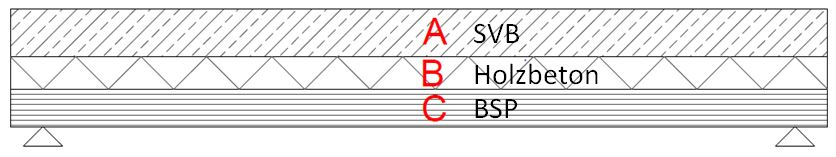
\includegraphics[scale =0.7]{sandwichaufbau.png}
\caption{Sandwichaufbau}
\label{sandwich}
\end{center}
\end{figure}

\subparagraph{Ziele und Vorgehensweise:}

Das erste übergeordnete Ziel dieser Arbeit ist die Entwicklung eines Sandwichaufbaus aus Brettsperrschichtholz (BSP), Holzbeton und selbeverdichtender Beton(SVB). Das zweite Ziel dieser Arbeit ist die Nachrechnung der Versuchsergebnisse mit den „$\gamma$ -Verfahren“ und dem Finite Elemente Programm „Sofistik“. Es sollen die Grundlagen zur Bemessung des Sandwichaufbaus entwickelt werden. 
Zusätzlich ist eine ökonomische Betrachtung des Sandwichaufbaus zu erstellen und einen Vergleich mit den gängigen Deckensystemen zu erarbeiten.\newline Die genannten Ziele sollen mit Hilfe von den experimentellen Großbauteilversuchen erzielt werden. Dabei wird ausschließlich das Kurzzeitverhalten des Sandwichaufbaus untersucht. Die Kurzzeitdurchbiegung wurde mit l/400 begrenzt, um für Langzeitverformungen Reserven zu generieren.




\newpage{}
Im Nachfolgenden Ablaufdiagramm ist die Vorgehensweise bei der Erstellung der Arbeit ersichtlich.

\begin{figure}[h]
\begin{center}
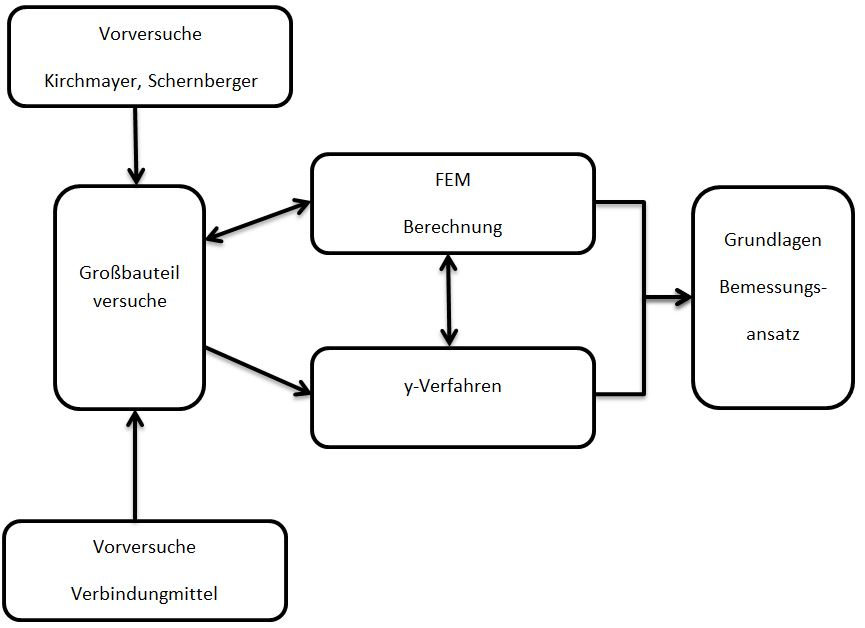
\includegraphics[scale =0.7]{ablauforganigramm.png}
\caption{Ablauforganigramm der Diplomarbeit}
\end{center}
\end{figure}




\section{Zusammenfassung der Kapitel}

\begin{enumerate}
\item Zusammenfassung von Vorarbeit 
\item Ermittlung der mechanischen Eigenschaften der Verbindungsmittel
\item Versuchaufbau und Durchführung
\item Beschreibung und Auswertung der Großbauteilversuche
\item Beschreibung der Berechnungsverfahren
\item Vergleich Berechnung Versuche und Berechnungen
\item wirtschaftliche Untersuchungen

\end{enumerate}




\chapter{Verbindungsmittel}

Man unterscheidet zwischen metallischen Verbindungsmitteln (Drahtstifte, Schrauben, Verbindungsbeschläge) und nichtmetallischen Verbindungsmitteln (Klebstoffe, Leime, Dübel, Federn).\footnote{http://www.sign-lang.uni-hamburg.de/tlex/lemmata/l7/l708.htm,[06,2013]}



\section{Schrauben}

Durch den ähnlichen Aufbau des Sandwiches zum Holzbetonverbund - System wurden die Verbundmöglichkeiten des Systems näher untersucht und für das Sandwich adaptiert. Das am häufigsten ausgeführte HBV-System wird mit Verbundschrauben direkt vor Ort hergestellt. Vorteil dieses Systems ist, das die Schrauben ohne Vorbohren in das Holz eingebohrt werden können. Es gibt mehrere Hersteller, die in der Arbeit von Schernberger [1] aufgelistet sind, die dieses System anbieten. Es wird auch auf die Einsatzmöglichkeiten und die Vor- und Nachteile jedes Herstellers eingegangen. 
Die Idee war, eine Verbindung zwischen Holz und Beton herzustellen, welche die Schubkräfte abtragen kann und damit den Holzleichtbeton unterstützt. Analog zum herkömmlichen HBV - System, wurde gemeinsam mit Firma SFS das System mit langen Holzschrauben als Schubverbinder entwickelt. Die Firma hat Schraubenreihen  in verschiedensten Ausführungsvarianten und entsprechenden Schraubenlängen. Um die Auswahl der Schrauben einzugrenzen, wurden folgende Eigenschaften vorgegeben:


\begin{enumerate} 
	\item Einschraubwinkel: $45^{\circ}$
	\item Schraubenlänge: 400 mm
	\item Einschraubtechnik: ohne Vorbohren
	\item Keine Beschädigung der Schrauben beim durchbohren des Holzleichtbetons (Velox)
\end{enumerate}


Der 4 Punkt war aufgrund des Sandwichaufbaus noch nicht überprüft worden. Daher wurden, in Zusammenarbeit mit der Firma SFS verschiedene Schraubentypen getestet. 

Die Schrauben unterschieden sich in: 

\begin{itemize}
	\item Schraubenkopfform
	\item Gewindeanordnung
	\item Schaftform
	\item Spitze
\end{itemize}

Ausgesuchte Schraubentypen: 


\begin{itemize}
	\item WR – dxL
	\item TWIN – DU dxL Sichel
	\item WT – T dxL 
	\item TWIN – DU dxL
	\item WR – T  dxL
\end{itemize}
	
\subsection{Schraubentype:	 WR – dxL}
Das Befestigungssystem WR findet hauptsächlich bei großen Querschnitten im Bereich der Verbindungen, Verstärkungen und Stahl-Holz-Anschlüsse, Anwendung. Die Schrauben sind aus Kohlenstoffstahl gefertigt. Der Schraubendurchmesser ist wählbar zwischen 9 mm oder 13 mm. Die Schrauben sind in den Längen von  250 mm bis 1000 mm verfügbar. Die Oberfläche der Schraube ist mit einem Durocoat überzogen, der als Korossionsschutz und als Gleitmittel fungiert.

\begin{figure}[h]
\begin{center}
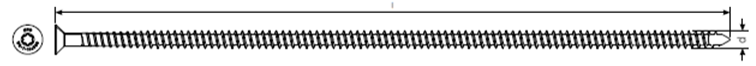
\includegraphics[scale =0.7]{WR-dxL.png}
\caption{Schraubentype: WR - dxL}
\end{center}
\end{figure}


\subparagraph{Positive Eigenschaften nach Hersteller[], sind:}

\begin{itemize}
	\item sehr hohe Leitungsfähigkeit
	\item breites Anwendungsspektrum
	\item Verschraubung auch paralell zur Faserrichtung möglich
	\item keine Abminderung der Tragfähigkeit von $90^\circ  -  45^\circ$ zur Faser
	\item Verarbeitung ohne Vorbohren
	\item geringe Spaltneigung
	\item unsichtbare Verbindung
\end{itemize}


\subsection{Schraubentype: TWIN-UD dxL Sichel }
Das System TWIN DU wird seit Jahren für die Befestigung von Aufsparrendämmung auf Dächern  und hinterlüftete Fassaden verwendet. Die Schrauben sind aus Kohlenstoffstahl gefertigt. Der Schraubendurchmesser beträgt 7,5 mm  und die Schraubenlänge variiert im Bereich von 160 mm bis 480 mm. Die Oberfläche der Schraube ist mit einem Durocoat überzogen, der als Korossionsschutz und als Gleitmittel fungiert.

\begin{figure}[h]
\begin{center}
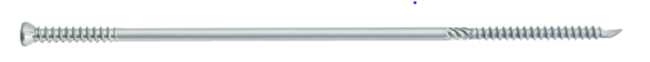
\includegraphics[scale =0.7]{TWIN-UDdxLSichel.png}
\caption{Schraubentype: TWIN-UD dxL Sichel}
\end{center}
\end{figure}


\subparagraph{Positive Eigenschaften nach Angaben des Herstellers [], sind:}

\begin{itemize}
	\item Holzbohrspitze reduziert die Spaltgefahr des 	Holzes
	\item optimiertes Doppelgewinde ohne		 Gangunterschied
	\item Rändel für erleichtertes Eindrehen
	\item mehr Leistung durch angepasste 	Gewindedurchmesser
	\item hohe Traglast auf Zug und Druck dank 	Doppelgewinde
	\item minimale Wärmebrücken bei vollflächiger 	Dämmung
	\item einfache Arbeitsschritte- minimaler 	Arbeitsaufwand
	\item Dämmstärken von 60 mm bis 300 mm möglich
\end{itemize}


\subsection{Schraubentype: WT – T dxL }
Das Befestigungssystem WT ist für den universellen Einsatz im konstruktiven Holzbau in Gebrauch. Die Schrauben sind aus Kohlenstoffstahl gefertigt. Der Schraubendurchmesser ist wählbar zwischen 6,5 mm oder 8,2 mm. Die Schrauben sind in den Längen von  65 mm bis 330 mm verfügbar. Die Oberfläche der Schraube ist mit einem Durocoat überzogen, der als Korossionsschutz und als Gleitmittel fungiert.

\begin{figure}[h]
\begin{center}
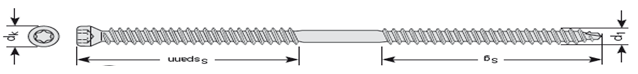
\includegraphics[scale =0.7]{WT-TdxL.png}
\caption{Schraubentype: WT-T dxL}
\end{center}
\end{figure}

\subparagraph{Positive Eigenschaften nach Hersteller[], sind:}

\begin{itemize}
	\item Einfache und sichere Berechnung
	\item Vielfältiges Anwendungsspektrum
	\item Dauerhafte Verbindung  bei hoher Tragfähigkeit
	\item Schnelles, effizientes Verarbeiten ohne Vorbohren
	\item Formschlüssige Verbindung  dank Doppelgewinde
	\item Hoher Brandwiderstand
	\item Anspruchsvolle Ästhetik dank versenkter Befestigungsmittel
	
\end{itemize}

\subsection{Schraubentype:	 WR – T  dxL}
Das Befestigungssystem WR-T ist für den universellen Einsatz im konstruktiven Holzbau in Gebrauch. Die Schrauben sind aus Kohlenstoffstahl gefertigt. Der Schraubendurchmesser ist wählbar zwischen 9 mm oder 13 mm. Die Schrauben sind in den Längen von  250 mm bis 1000 mm verfügbar. 

\begin{figure}[h]
\begin{center}
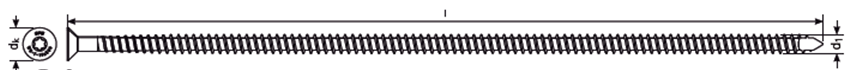
\includegraphics[scale =0.7]{WR-TdxL.png}
\caption{Schraubentype: WT-T dxL}
\end{center}
\end{figure}

\subparagraph{Positive Eigenschaften nach Angaben des Herstellers [], sind:}

\begin{itemize}
	\item hohe Tragfähigkeit
	\item einfache Verarbeitung
	\item hoher Brandwiderstand der Verbindung
	\item schnelle Montage ohne Vorbohen
	\item Verbindungsmittel nicht sichtbar
\end{itemize}

\subsection{Versuchsaufbau für Schrauben}

Bei der Produktion werden zuerst die Holzbetonplatten auf die BSP geklebt und anschließend die Schrauben durch die Holzbetonplatten in die BSP eingeschraubt. Die Versuchsdurchführungen sollen sicher stellen, dass nach der Durchdringung der Holzleichtbetonschicht, das Gewinde und die Spitze keinen Schaden nehmen und damit eine einwandfreie Verbindung im Holz zustande kommt. \newline Es wurden 4 Lagen Veloxplatten zu je 5cm übereinandergelegt und mit Klemmzangen zusammengehalten. Um das Durchbohren und die anschließende Besichtigung der Schrauben zu ermöglichen, wurden die Platten auf Holzböcken gelagert.  

\begin{figure}
\begin{center}
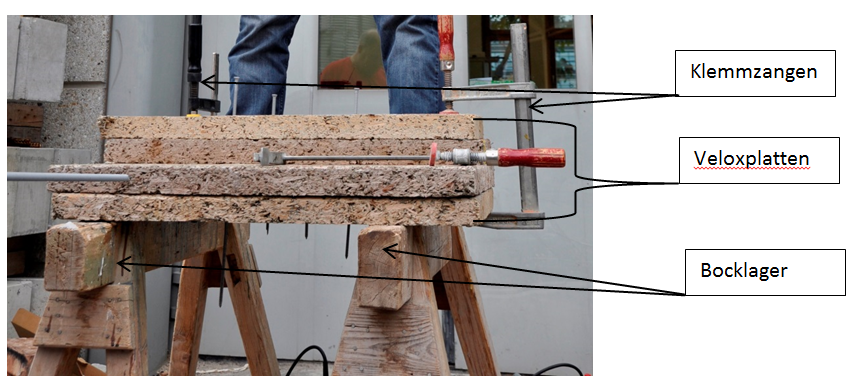
\includegraphics[scale =0.6]{Schraubenversuchsaufbau.png}
\caption{ Schraubenversuchsaufbau}
\end{center}
\end{figure}

\subsection{Versuchsauswertung}

In Abbildung \ref{Schraubenauswertung} sind die Schraubenspitzen nach dem Durchbohren der Veloxplatten dargestellt. Es ist ersichtlich, dass keine der Schrauben beschädigt worden ist. Weiters war beim Einbohren der Schrauben, kein Unterschied im Kraftaufwand festzustellen. 

\begin{figure}[h!]
\begin{center}
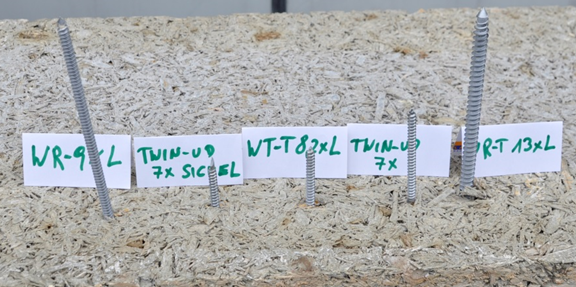
\includegraphics[scale =0.8]{Schraubenauswertung.png}
\caption{ Schraubenwertung}
\label{Schraubenauswertung}
\end{center}
\end{figure}



Die Auswahl der Schraube erfolgte Aufgrund der folgenden Kriterien.
Um über den gesamten Einbohrvorgang eine Führung zu gewährleisten, wurde eine Gewindeanordnung über die gesamte Schraubenlänge bevorzugt. Zusätzlich kann durch das Gewinde, ein besserer Auszugswiderstand aus dem Beton gewährleistet werden. Die Bandbreite der Schraubenlänge beträgt 250 mm bis 1000 mm.
Die Spitze war ein weiteres Entscheidungskriterium, hierbei wurde darauf geachtet, dass sich die Schraube problemlos mit einem einfachen Hilfsmittel (Hammer) ansetzen ist. 
Der Schraubenkopf sollte eine große Fläche vorweisen, damit ein guter  Verbund mit dem Beton entsteht. 
Durch die Vorgabe, von einer lichten Weite bis zu 10 m und damit die einhergehende Bauteilerhöhung muss auch die Schraubenlänge noch erweiterbar sein.
\newline{}

Alle Kriterien erfüllte die Schraubentype: \textbf{WR – T dxL} 




\section{Kleber}
Unter Kleben (nach EN DIN 923,[]) versteht man: Fügen gleicher oder ungleicher Werkstoffe unter Verwendung eines Klebstoffes. 

Klebstoffe sind (nach EN DIN 923,[]) nichtmetallische Stoffe, die Fügeteile durch Flächenhaftung und innere Festigkeit(Adhäsion und Kohäsion) verbinden.


\subsection{Einteilung}

Die Einteilung der Klebestoffe wird in Habenicht[] auf zwei Arten angeführt. Zum einem auf der chemischen Basis und nach dem Abbindemechanismus. 
\begin{figure}[h]
\begin{center}
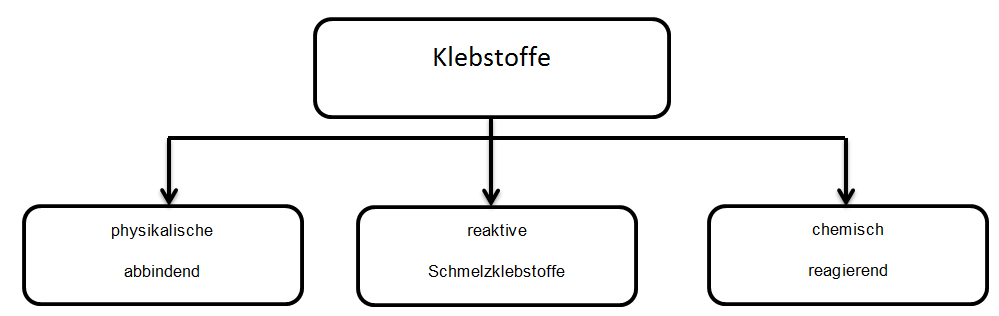
\includegraphics[scale =0.6]{einteilungderklebstoffe.png}
\caption{ Einteilung der Klebstoffe nach dem Abbindemechanismus, []}
\label{Einteilung der Kelbstoffe}
\end{center}
\end{figure}


\subsection{Vor- und Nachteile der Klebverbindungen}

Habenich [] hat die Vor- und Nachteile des Klebens gegenüber Schweißen, Löten, Schrauben, und Nieten beschrieben. 
\newline{}

\textbf{Vorteile von Klebungen,[4, Tabelle 7.1]}
\begin{itemize}
	\item gleichmäßige Spannungsverteilung senkrecht zur Belastungsrichtung 
	\item keine Thermische Gefügebeeinflussung
	\item kein thermisch bedingter Bauteilverzug
	\item Verbindungsmöglichkeit für unterschiedliche Materialkomponenten
	\item Gewichtsersparnis, Leichtbau
	\item Verbingungsmöglichkeit für sehr wärmeempfindliche Werkstoffe
	\item Festigkeitserhöhung in Verbindung mit Schrauben
	\item hohe dynamische Festigkeit, hohe Schwingunsdämpfung
	\item Möglichkeit zur Automatisierung
\end{itemize}


\textbf{Nachteile von Klebungen, [4, Tabelle 7.2]}

\begin{itemize}
	\item Einfluss der Zeit auf den Verfahrensablauf
	\item Oberflächenvorbehandlung der Fügeteile
	\item begrenzte thermische Frombeständigkeit
	\item sorgfältige Prozesskontrolle
	\item Alterungsabhängigkeit der Klebschicht und Grenzschicht
	\item aufwendige Kontrollverfahren
	\item geringe Schälwiderstände, Kriechneigung
	\item begrenzte Reparaturmöglichkeiten
	\item aufwendige Festigkeitsberechnungen
	\item Demontage von Klebungen
	\end{itemize}

Bei der Auflistung der Vor -und Nachteile können die Nachteile durch die vorgesehene Verwendung fast alle entschärft werden. Die Vorteile der Verbindungsmethode sind zumeist zutreffend. Aus diesen Überlegungen ist die Anwendung der Klebeverbindung beim Sandwichbauteil gerechtfertigt.



\subsection{Ermittlung des Kleberbedarfs mit der Sandfleckmethode}

Mit der Sandfleckmethode wird die Rauigkeit von porösen Materialien bestimmt  
und mit einem Formelwerk der Bedarf ermittelt.

\paragraph{Durchführung}
Es wird 15 $g$ feiner Sand mit eine Körnung von 0,1 - 0,2 $mm$ in einen kleinen Behälter gefüllt. Anschließend wird der Sand auf dem porösem Material aufgebracht [Abbildung \ref{sandfleck}]und mit Hilfe eines Stempels kreisförmig verteilt. Somit werden die oberflächigen Hohlräume (Poren) ausgefüllt. Der mittlere Durchmesser des „Sandflecks“ wird anschließend gemessen [Abbildung \ref{sandfleckmessen}]. Anhand des Durchmesser und des Volumens wird die Rautiefe bestimmt. Mit Rautiefe und zusätzlichen Parametern (Spachtelfaktor, Schichtdicke) wird der Kleberverbrauch berechnet.

\begin{figure}[h]
\begin{minipage}[hbt]{7cm}	
	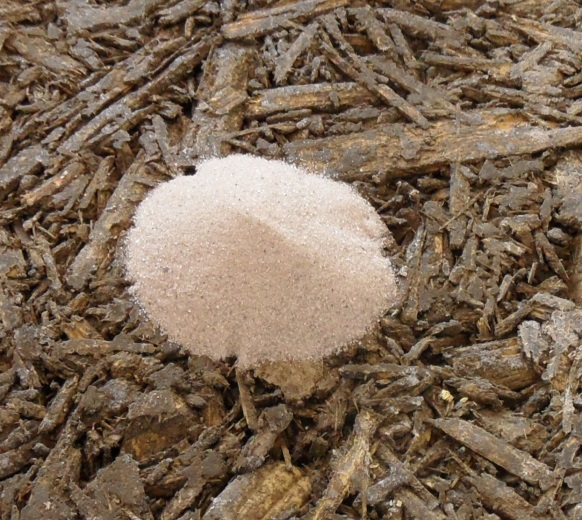
\includegraphics[width=7.7cm]{sandfleck.png}
	\caption{Aufgeschütteter Sandfleck}
	\label{sandfleck}
\end{minipage}
\hfill
\begin{minipage}[hbt]{7cm}
	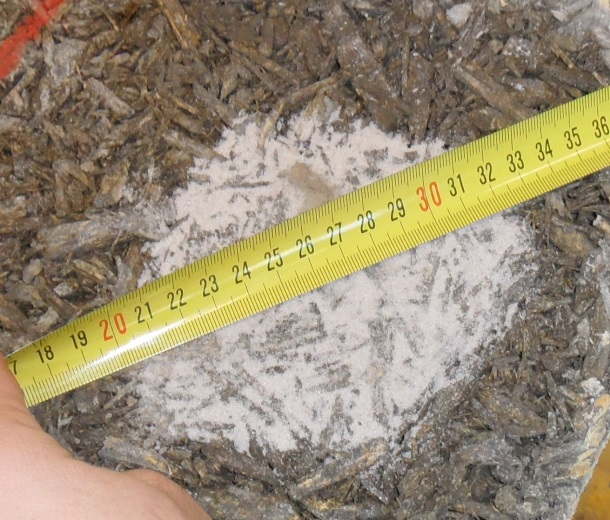
\includegraphics[width=8cm]{sandfleckmessen.png}
	\caption{Ermittlung des mittleren Durchmessers}
	\label{sandfleckmessen}
\end{minipage}
\end{figure}
\paragraph{Berechnng des Kleberbedarfs: SikaTop-109 ElastoCem, nach Sika}

\textbf{Angaben:}
\begin{center}

\begin{itemize}
\item mittlere Durchmesser:D=11$cm$
\item Sandvolumen:	V=0,01$L$
\item Dichte:	$\rho$=1.60 $\frac{kg}{L}$
\item Trägerabmessung(l x b):	7,40 x 0,50 $m $
\end{itemize}
\end{center}


\textbf{Annahmen:}

\begin{itemize}
\item Spachtelfaktor:	$f_{sp}=\dfrac{2}{3}$
\item Schichtdicke:		$f_{sd}=3mm$
\end{itemize}
 

\subparagraph{Berechnung der Rauigkeit:}
\begin{equation}
r=\dfrac{V*4}{\pi*d^{2}}=1,052 mm
\end{equation}

\subparagraph{Kleberbedarf pro Fläche}

\begin{equation}
b_{K}= 2\dfrac{kg}{L}*f_{sd}=6\dfrac{kg}{m^{2}}
\end{equation}

\subparagraph{Kleberbedarf für Porenverschluss}

\begin{equation}
b_{K,P}=r*\rho*f_{sd}= 1,122\dfrac{kg}{m^{2}}
\end{equation}

\subparagraph{Bedarf für CLT-Velox-Schichte}

\begin{equation}
B_{CLT-Velox}=Kb*l*b=22,22 kg
\end{equation}

\subparagraph{Bedarf für Velox-Velox-Schichte}

\begin{equation}
B_{Velox-Velox}=(Kb+Kp)*l*b=26,35 kg
\end{equation}


\subparagraph{Benötigter Kleber für den gesamten Träger}

\begin{equation}
B_{gesamt}=B_{CLT-Velox}+2*B_{Velox-Velox}=74,91 kg
\end{equation}




\subsection{Kleberversuchsreihe 1}

Beim 1 Großbauteilversuch traten einige Probleme bei der Verarbeitung des Kleber Sikadur 31 auf. Dieser Kleber wurde auch von Kirchmayer bei seinen Verbundversuchen verwendet. Da der Aufbau von Kirchmayer kleiner war und somit auch die Klebermenge geringer, hatte er keine Probleme bei der der Verarbeitung. Der Kleber entwickelt bei großen Mischmengen eine schnelle Aushärtezeit und war beim Auftragen über den gesamten Träger sehr schwer zu Verarbeiten. Dies war auch bei der Ansicht, von Teilen des Versuchskörpers ersichtlich. In der Abbildung \ref{kleberfoto} sind größere Teilflächen zu erkennen, auf denen keine oder nur geringe Spuren des Veloxmaterials haften blieb. Dies ist auf die ungenügende Verarbeitung zurückzuführen. Um den eine bessere Verarbeitung zu gewährleisten und wirtschaftlichere Kleber zu verwenden, wurden alternative und kostengünstigere Kleber untersucht. 
\begin{figure}[h]
\begin{center}
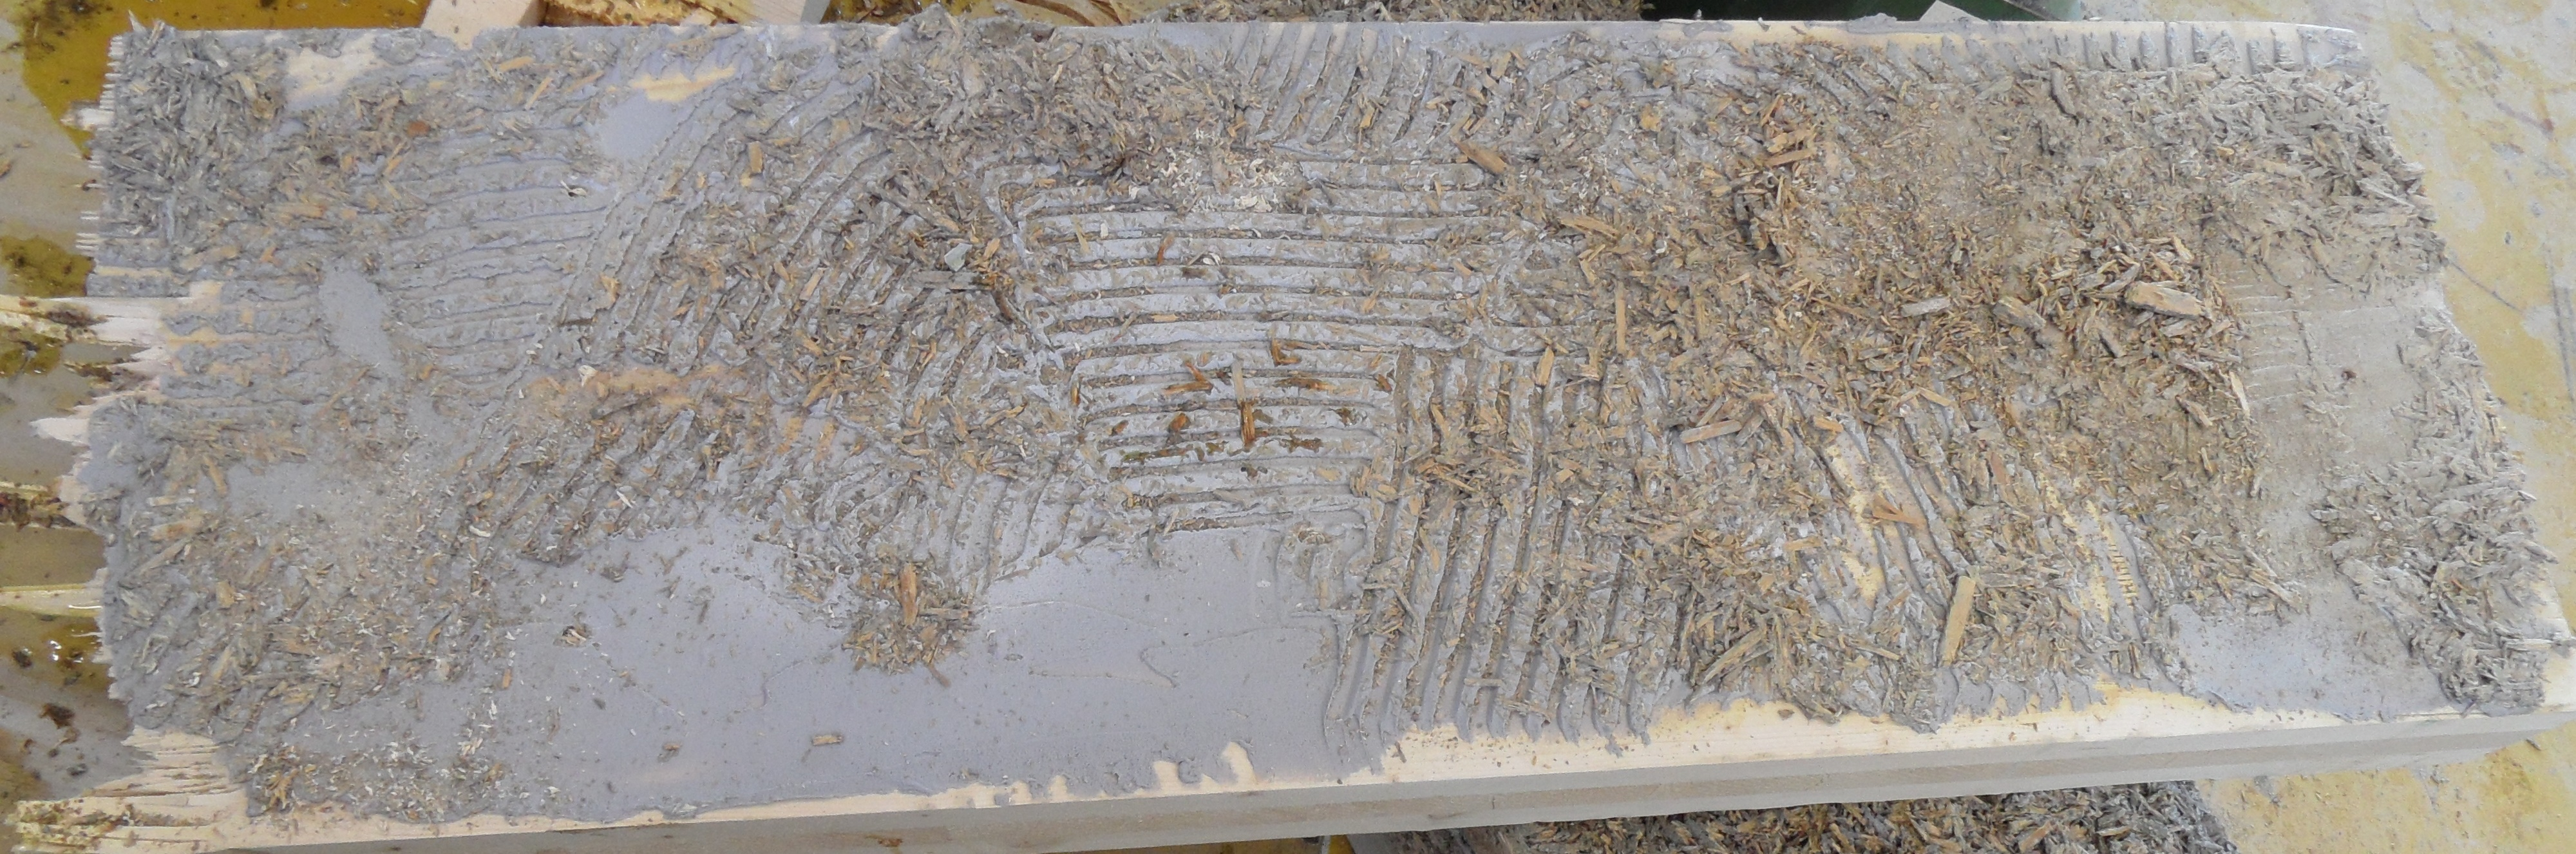
\includegraphics[scale =0.1]{kleberfoto.jpg}
\caption{ Verbundfäche von der Kleberschicht: BSP-Velox}
\label{kleberfoto}
\end{center}
\end{figure}



In Abstimmung mit der Firma Sika wurde die Anwendung abgeklärt und folgende Kleber getestet:
\begin{itemize}
\item Sikafloor 161
\item ElastoCem 109
\item SikaForce 7710 L35
\end{itemize}


auf folgende Eigenschaften der Kleber wurde näher eingegangen :	

\begin{itemize}
\item Verarbeitbarkeit
\item Haftzug
\item Verbrauch
\end{itemize}


\subparagraph{Anmischen:}
Die untersuchten Kleber basieren alle au einem 2- Komponenten-System. Daher mussten die Komponenten nach dem vom Hersteller  angegebenen Mischverhältnis abgemischt werden. Um eine einheitliche Masse zu erhalten, wurden die 2 Komponenten mit einem Quirl vermischt. Der Kleber Sikafloor 161 wurde noch zusätzlich mit einem Thixotropierungsmittel verarbeitet.

\subparagraph{Auftragen:}
Zuerst wurden die oberflächigen Poren vom Holzbeton (Velox) mit Hilfe einer Spachtel verschlossen. Anschließend wurde der Kleber mit einer Zahnspachtel aufgetragen.

\section{Haftzugprüfung}
Um den Verbund der Kleber mit der Veloxplatte zu untersuchen, wurde die Haftzugprüfung angewendet.
Die Haftzugprüfung  wurde mit den angeführten Klebern durchgeführt. Zusätzlich wurde eine Prüfung ohne Kleber (nur auf das Velox) durchgeführt, um einen Referenzwert zu erhalten. In der Abbildung \ref{Z16E} ist das Prüfeinheit dargestellt.

\begin{figure}
\begin{center}
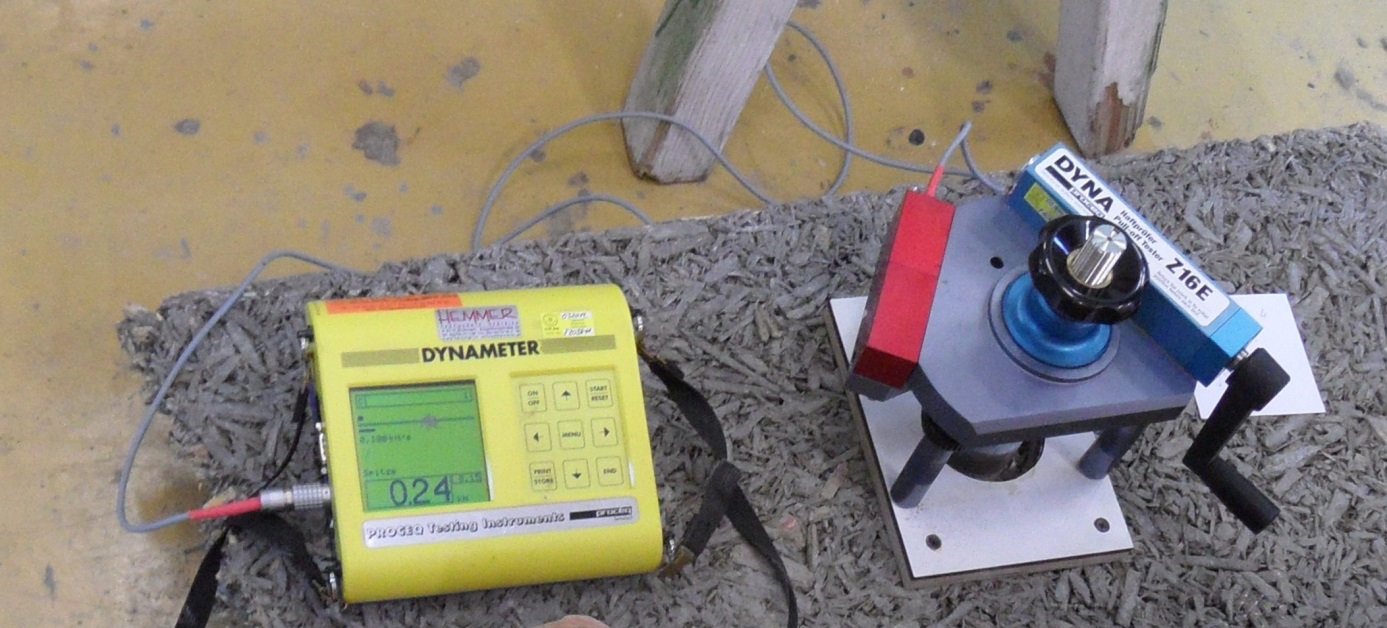
\includegraphics[scale =0.7]{Z16E.jpg}
\caption{ Prüfgerät:Dynameter Z16E}
\label{Z16E}
\end{center}
\end{figure}

\newpage{}

\subsection{Versuchsvorbereitung}

\begin{enumerate}
\item Anmischen des 2 Komponentkleber
\item Auftragen der Kleber auf das Velox.
\item Aushärtezeit:  1 Woche
\item 3 Kernbohrungen wurden auf jeden Versuchskörper aufgebracht
\item Aufwärmen der Prüfstempel (Beschleunigung der Aushärtung)
\item Abmischen des Klebers des Klebers für die Kraftübertragung zwischen dem Stempel und den Testkleber
\item Auftragen des Klebers (Uhuplus oder X60)
\item Aufbringen des vorgewärmten Prüfstempels
\item Aushärten des abgemischten Klebers (15 min oder 4 min)
\end{enumerate}

\newpage{}
In den nachfolgenden Abbildungen \ref{1Versuchsplatte} - \ref{4Versuchsplatte} sind die getrockneten Kleber und die aufgeklebten Prüfstempel ersichtlich.

\begin{figure}[h]
\begin{minipage}[hbt]{7cm}	
	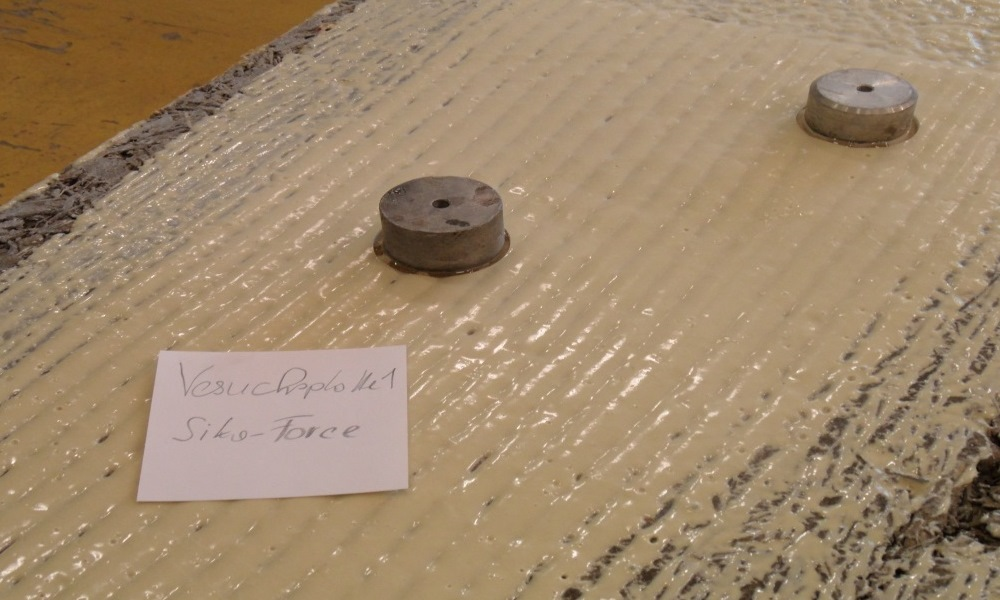
\includegraphics[width=7cm]{1Versuchsplatte.jpg}
	\caption{Versuchsplatte (Sika-Force 7710 L35)}
	\label{1Versuchsplatte}
\end{minipage}
\hfill
\begin{minipage}[hbt]{7cm}
	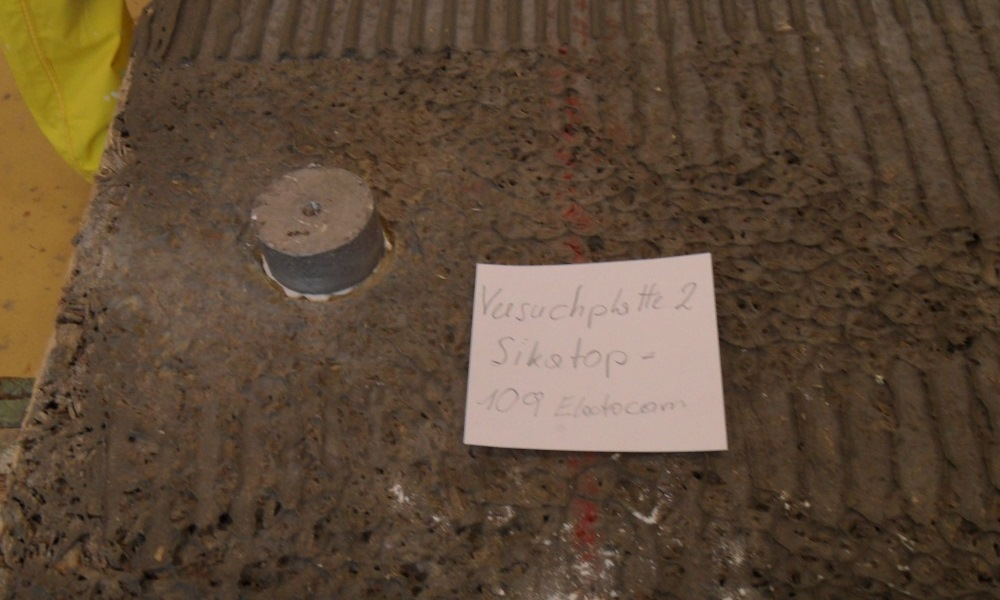
\includegraphics[width=7cm]{2Versuchsplatte.jpg}
	\caption{Versuchsplatte (Sikatop-109 Elastocam)}
	\label{2Versuchsplatte}
\end{minipage}
\end{figure}


\begin{figure}[h]
\begin{minipage}[hbt]{7cm}	
	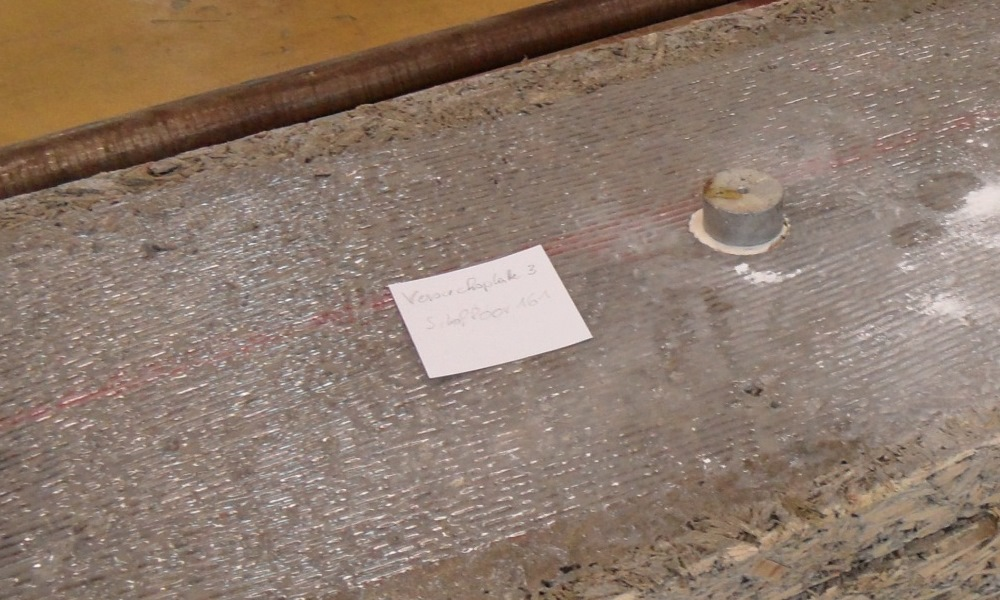
\includegraphics[width=7cm]{3Versuchsplatte.jpg}
	\caption{Versuchsplatte (Sikafloor 161))}
	\label{3Versuchsplatte}
\end{minipage}
\hfill
\begin{minipage}[hbt]{7cm}
	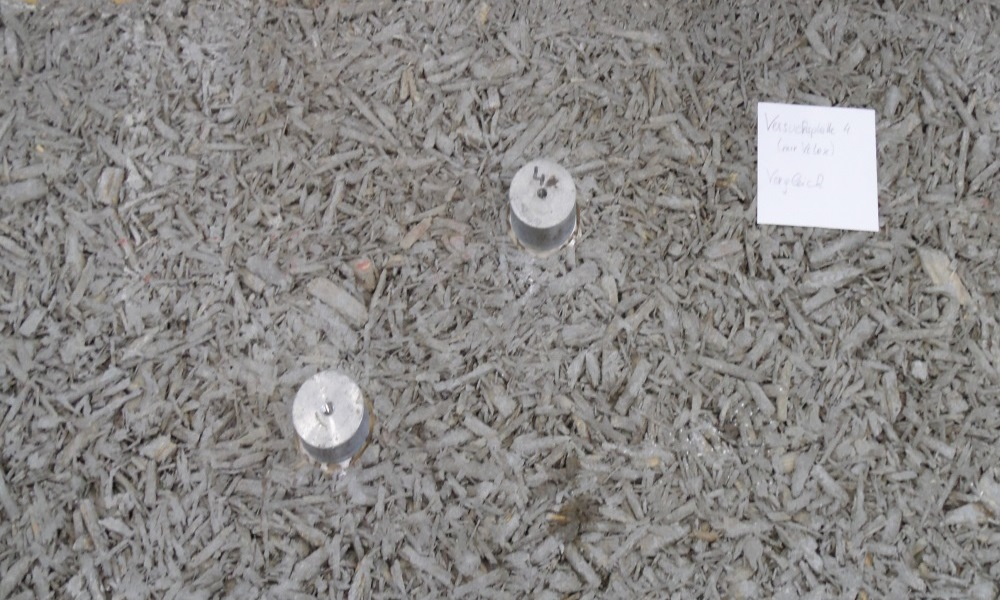
\includegraphics[width=7cm]{4Versuchsplatte.jpg}
	\caption{Versuchsplatte (ohne Kleber)}
	\label{4Versuchsplatte}
\end{minipage}
\end{figure}

\subsection{Versuchsdurchführung}

\begin{enumerate}
\item Einschrauben des Bolzens in den Stempel
\item Aufstellen des Haftzugprüfgeräts (Dynameter Z16E)
\item Einfädeln des Bolzens in die Einkerbung
\item manuelles Kraftaufbringen durch die Handkurbel
\item Ablesen der max. Kraft auf dem Messgerät
\end{enumerate}

In der Abbildung \ref{dynameter} ist die Messeinheit mit den beschrifteten Hauptbestandteilen dargestellt. 

\begin{figure}
\begin{center}
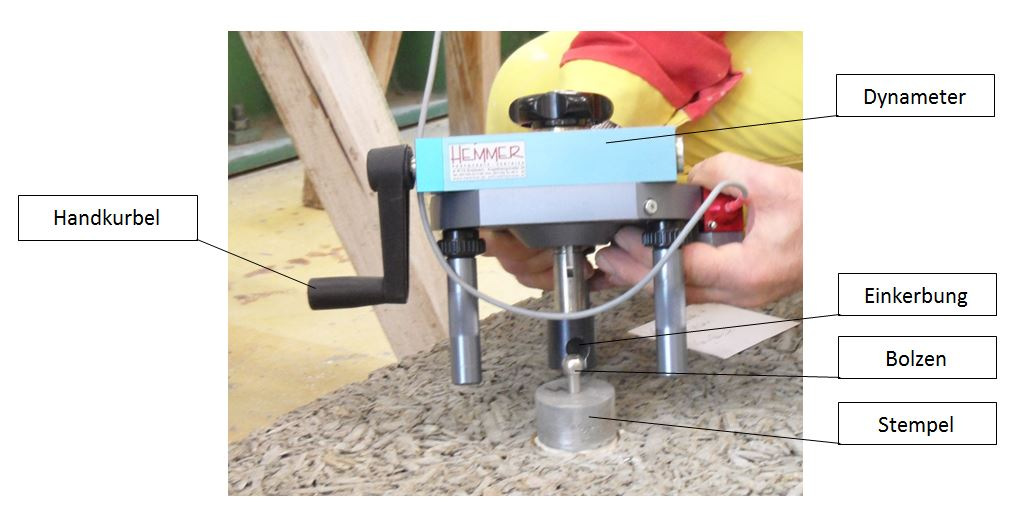
\includegraphics[scale =0.6]{dynameter.jpg}
\caption{ Dynameter Z16E}
\label{dynameter}
\end{center}
\end{figure}



\begin{table}
\caption{Messergebnisse Haftzugprüfung}
\begin{center}

\begin{tabular}{|c|c|c|c|c|} \hline
Versuchsplatte & Kraft & Durchschnitt & Spannung &Durchschnitt \\

	& [kN] & [kN] & [N/mm$^{2}$] & [N/mm$^{2}$] \\
	\hline\hline
 \cline{2-2} 1 Versuch: Sika Force  & 1,47 & & 0,75& \\\cline{2-2}&1,56 &1,45 &0,79 &0,74 \\\cline{2-2}&1,32 & &0,67 & 
\\\hline\hline

 \cline{2-2} 2 Versuch: Sikatop 109  & 0,74 & & 0,38& \\\cline{2-2}&0,77 &0,77 &0,39 &0,39 \\\cline{2-2}&0,80 & &0,41 & 
\\\hline\hline

 \cline{2-2} 3 Versuch: Sikafloor 161  & 2,11 & & 1,07& \\\cline{2-2}&1,82 &2,04 &0,93 &1,04 \\\cline{2-2}&2,20 & &2,12 & 
\\\hline\hline


 \cline{2-2} 4 Versuch: nur Velox  & 0,84 & & 0,43& \\\cline{2-2}&0.80 &0,82 &0,41 &0,42 
\\\hline

\end{tabular}
 \label{tab:1 kleberversuche}

\end{center}
\end{table}




\textbf{Zwischenfazit:}
\newline

Die Kleber Sika Force und Sikafloor 161 haben sehr gute Klebeeigenschaft, die man anhand der Versuchsergebnisse \ref{tab:1 kleberversuche} erkennen kann. Es versagte bei den beiden nicht der Kleber sondern das Velox. Die innere Festigkeit vom Velox war geringer, als die des Klebers. 

Beim Kleber Sikatop hat nicht das Velox versagt, sondern der Kleber. Es ist zu vermuten, dass das Velox eine höhere innere Festigkeit hat als der Kleber hat. Da der Kleber ElastoCem 109 auf Zementbasis basiert, ist eine Aushärtezeit von 28 Tagen erforderlich, damit er seine Endfestigkeit erreicht.  Somit werden die Ergebnisse der Haftzugprüfung nach einer Woche unterschätzt.  Die Haftzugfestigkeit wird im Produktdatenblatt der Fa. Sika mit 0,7 N/$mm^{2}$ geführt. Daher ist zu erwarten, dass die innere Festigkeit des Klebers mit längerer Aushärtezeit ansteigt.
Aufgrund der einfachen Vorbereitung und der guten Verarbeitung haben wir uns für den Kleber \textbf{ElastoCem 109} für den Sandwichbauteil entschieden. Die innere Festigkeit sollte laut dem Produktdatenblatt[] nach entsprechender Aushärtezeit, höher als die die vom Velox sein. Durch die Verwendung des Aufbetons muss eine entsprechende Aushärtezeit für den Bauteil vorgesehen werden und ergibt daher die keine Einschränkung für den Kleber. 



\subsection{2 Kleberversuchsreihe}

Es wurden nach dem 2 Großbauteilversuch weitere Kleberversuche durchgeführt. Der Grund war, dass der Kleber ElastoCem 109 schon beim einheben in die Prüfeintichtung Beschädigungen aufwies. Es waren schon Teile der Veloxschichten nicht mehr miteinander verbunden. Dies war vor allem bei den Auflager ersichtlich. Durch den nicht vorhandenen Verbund waren auch Zugrisse in der Aufbetonschicht aufgetretten. In den Abildungen \ref{lagera} und \ref{lagerb} ist dargestellt, in welchen Ausmaß sich die Veloxplatten von einander lösten. Die Messlatte war 30 $ cm $ lang und die Unterteilungen kennzeichnen 5 $ cm $ Schritte.  

\begin{figure} [h]
\begin{minipage}[hbt]{7cm}	
	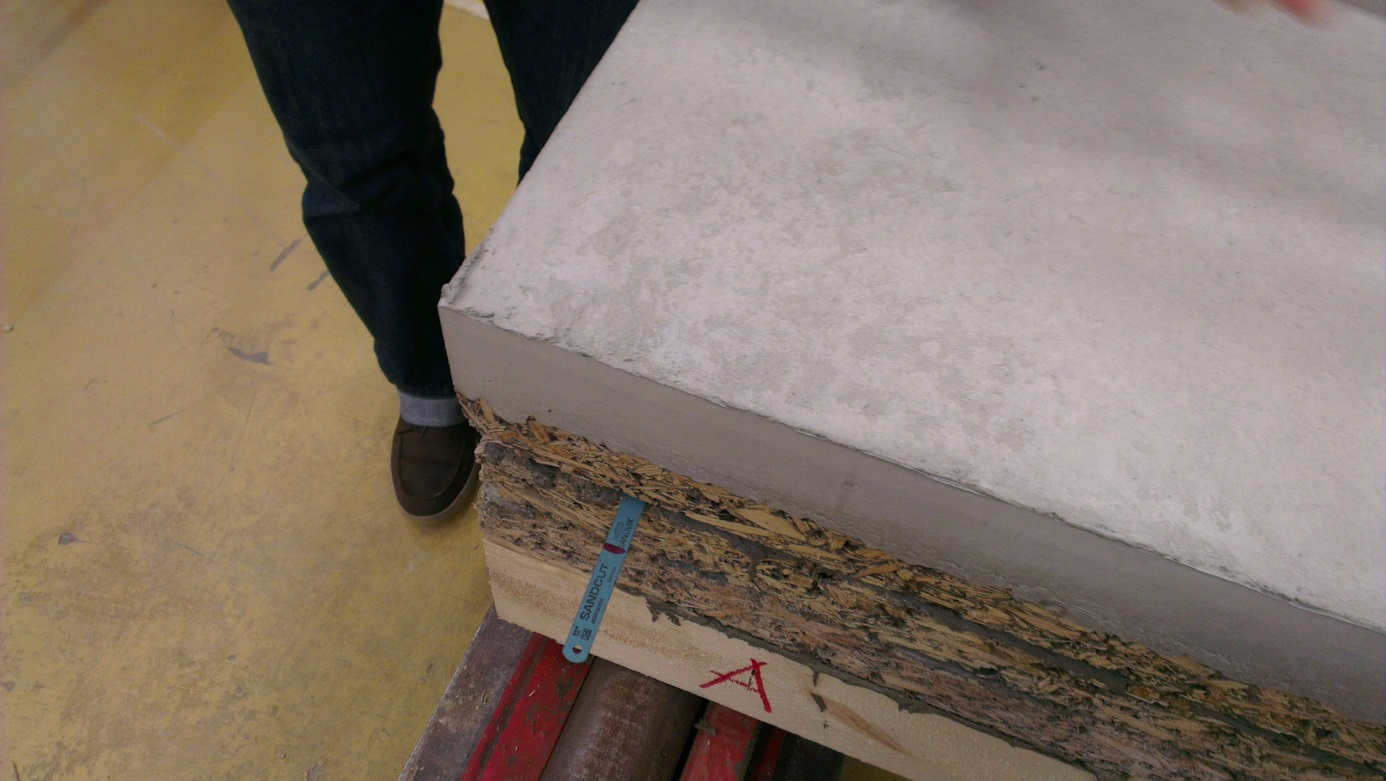
\includegraphics[width=7.7cm]{lagera.jpg}
	\caption{Verbundlosigkeit beim Auflager A}
	\label{lagera}
\end{minipage}
\hfill
\begin{minipage}[hbt]{7cm}
	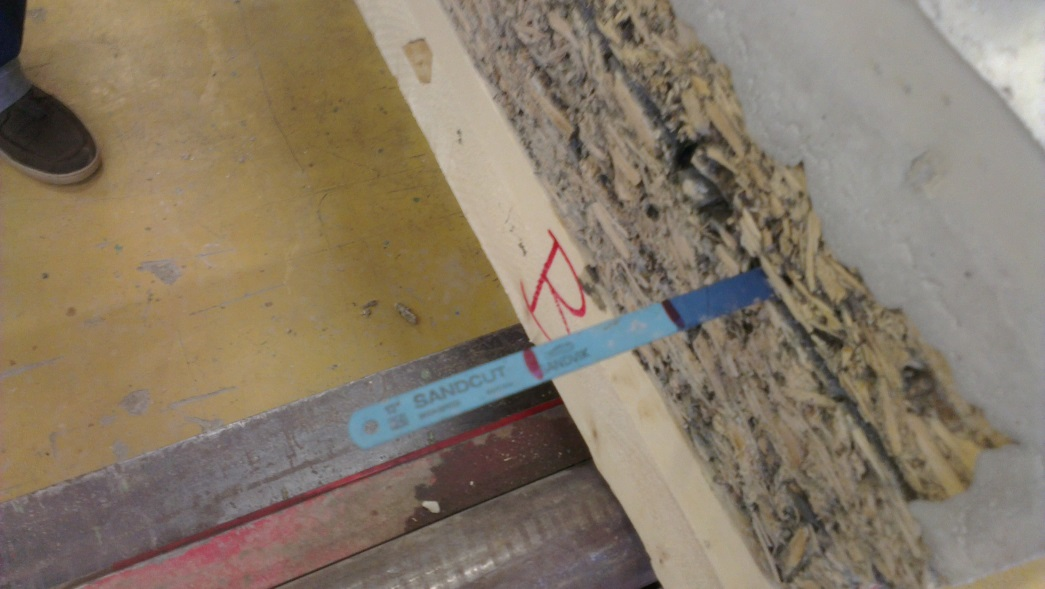
\includegraphics[width=8cm]{lagerb.jpg}
	\caption{Verbunglosigkeit beim Lager B}
	\label{lagerb}
\end{minipage}
\end{figure}



Es wurde wieder in der Absprache mit der Firma Sika ein  2- Komponenten Kleber  SikaTop 107 gewählt. Dieser Kleber hat etwa die doppelte Festigkeit (lt.Produktdatenblatt[]) des Kleber ElastoCem 109. Er besitzt die gleichen Verarbeitungsvorteile wie der Kleber ElastoCem 109.
 Um das Verbundverhalten des Klebers mit dem CLT-Holz zu untersuchen, wurden Versuchsproben erstellt. Der Aufbau und Ablauf entsprach der Versuchreihe in Abschnitt [Haftzugprufung] Versuchsreihe.
In Abbildungen \ref{holz-kleber} und \ref{velox-kleber} sind die Versuchskörper für das BSP (H1-H3) und für das Velox (V1-V3) dargestellt.


\begin{figure} 
\begin{minipage}[hbt]{7cm}	
	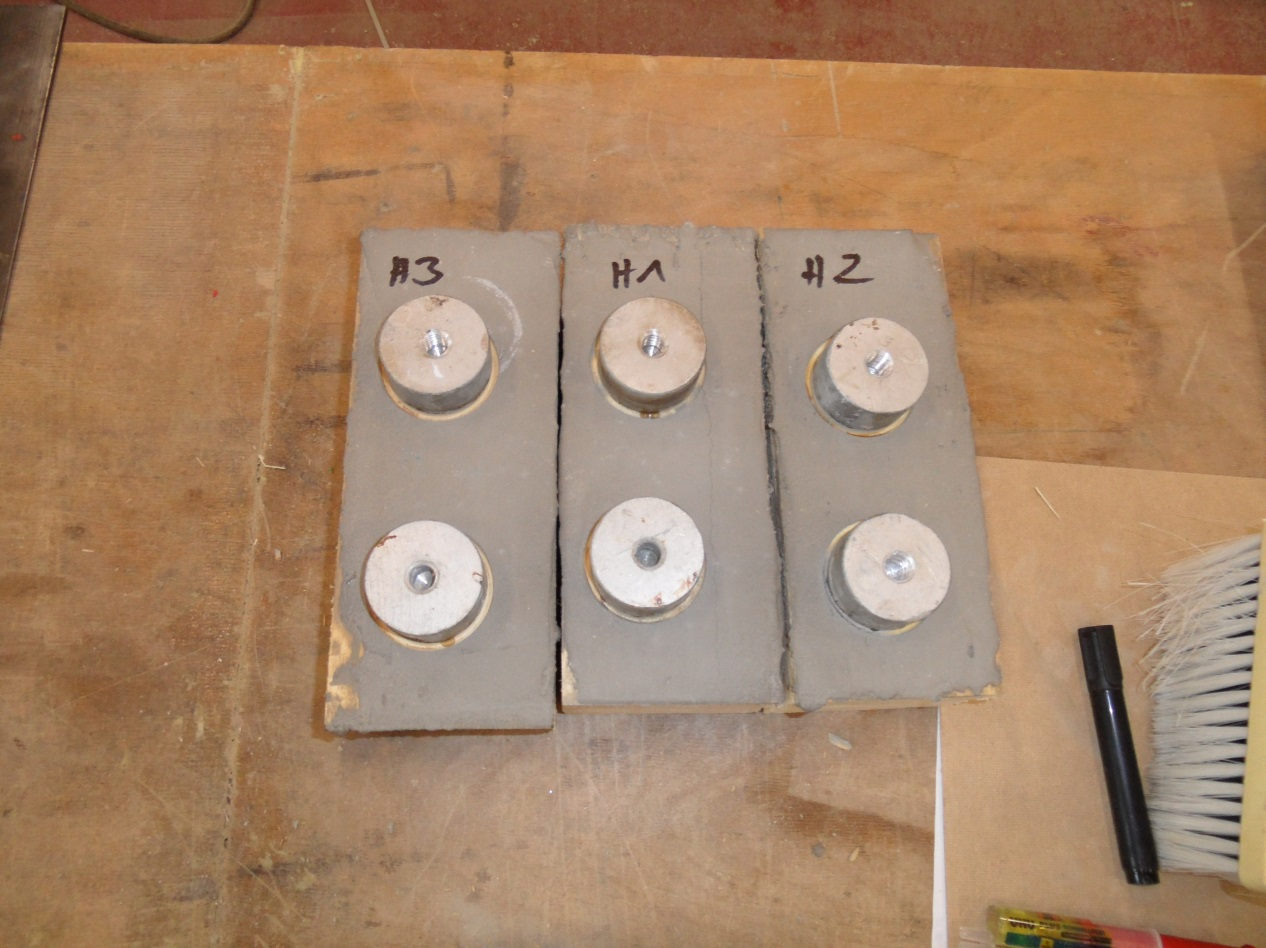
\includegraphics[width=7.7cm]{holz-kleber.jpg}
	\caption{Versuchskörper: Sikatop 107 auf Holz}
	\label{holz-kleber}
\end{minipage}
\hfill
\begin{minipage}[hbt]{7cm}
	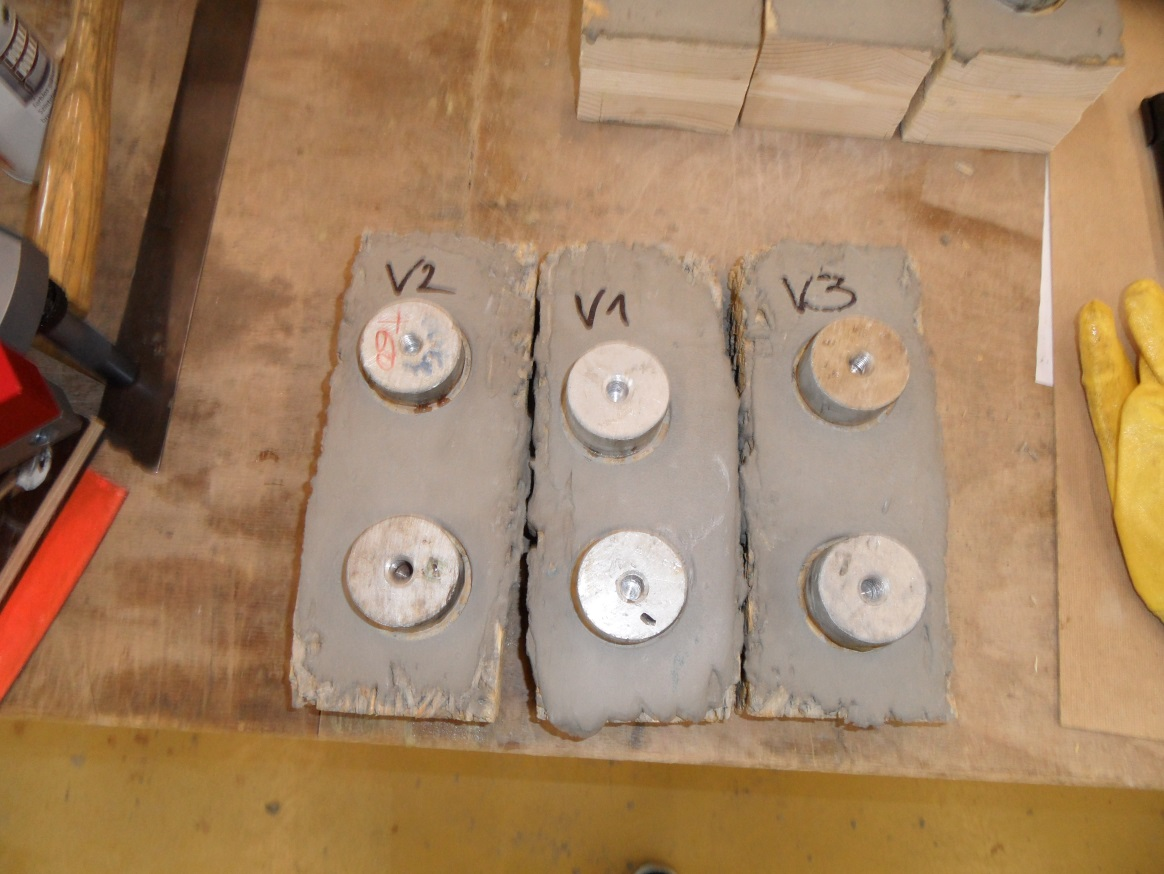
\includegraphics[width=8cm]{velox-kleber.jpg}
	\caption{Versuchskörper: Sikatop auf Velox}
	\label{velox-kleber}
\end{minipage}
\end{figure}

Der Kleber Sikatop 107 wurde mit dem Mischverhältnis von 1:4,5 abgemischt und auf die Probenkörper aufgetragen. Vor dem Auftrag wurde das Holz und das Velox noch befeuchtet, da beim aushärten des Klebers ein Feuchtigkeitstransport in das Holz stattfindet. Um einen Vergleich zu der ersten Versuchsreihe zu erhalten, härtete der ebenfalls eine Woche aus. Der Ablauf der Haftzugprüfung erfolgte ident zu den vorigen Versuchen.

In Abbildung \ref{probenbild} sind die Proben mit den dazugehörigen Bruchflächen dargestellt. Einige Stempel weisen rot markierte Stellen auf, da in diesem Bereich der schnellhärtende Epoxidkleber (UHU-Plus) nicht geklebt hat. Daher wurde bei der Spannungsberechnung die Fläche (D = 5cm) um diesen Anteil abgemindert. [Tabelle:\ref{tab:2.1 kleberversuche}]

\begin{figure}
\begin{center}
\includegraphics[scale =0.8]{Probenbild.jpg}
\caption{Bruchflächen der Proben (SikaTop 107); rote Markierung: fehlender Verbund zwischen schnellhärtenden Epoxidkleber und Stempel}
\label{probenbild}
\end{center}
\end{figure}





\begin{table}
\caption{Auswertung der 2 Kleberversuchsreihe, CLT}
\begin{tabular}{|c|c|c|c|c|c|} \hline
\multicolumn{6}{|c|}{Sikatop auf CLT} \\\hline
Versuchsplatte & Kraft & Durchschnitt & Spannung & Abminderung & Durchschnitt \\
	& [kN] & [kN] & [N/mm$^{2}$] & [\%] & [N/mm$^{2}$] \\
	\hline\hline
\cline{2-2} 1 Versuch: H1  & 1,25 & & 0,85& 25,0& \\\cline{2-2}&0,99 & 1,12 &1,51 & & 1,18
\\\hline\hline

\cline{2-2} 2 Versuch: H2  & 1,46 & & 1,30& 43,0& \\\cline{2-2}&1,86 & 1,66 &0,95 & & 1,13
\\\hline\hline

\cline{2-2} 3 Versuch: H3 & 1,07 & & 0,62&12,0 & \\\cline{2-2}&2,27 &1,67 &1,16 & 5,0 & 0,89 
\\\hline

\end{tabular}
 \label{tab:2.1 kleberversuche}
 \end{table}

\begin{table}
\caption{Auswertung der 2 Kleberversuchsreihe, Velox}
\begin{center}


\begin{tabular}{|c|c|c|c|c|} \hline
\multicolumn{5}{|c|}{Sikatop auf Velox} \\\hline
Versuchsplatte & Kraft & Durchschnitt & Spannung & Durchschnitt \\
	& [kN] & [kN] & [N/mm$^{2}$] & [N/mm$^{2}$] \\
	\hline\hline
\cline{2-2} 1 Versuch: V1  & 0,34 & & 0,17& 0,0 \\\cline{2-2}&0,56 & 0,46 &0,30 &0,23
\\\hline\hline

\cline{2-2} 2 Versuch: V2  & 0,52 & & 0,26 & 0,0 \\\cline{2-2}&0,39 & 0,46 &0,20 & 0,23
\\\hline\hline

\cline{2-2} 3 Versuch: V3 & 0,26 & & 0,13 & \\\cline{2-2}&0,64 & 0,45 & 0,33 & 0,23  
\\\hline
\end{tabular}

\label{tab:2.2kleberversuche}

\end{center}
\end{table}


\newpage{}

\paragraph{Fazit:}

Die Versuchsergebnisse weisen eine starke Streuung auf. Bei Versuch V3 beträgt der Messwert der zweiten Probe mehr als das Doppelte der ersten Messung. Berechnet man jedoch einen Mittelwert, weichen die Werte kaum voneinander ab. Hier ist auch ersichtlich, für die Haftzugversuche mit Velox, dass bei jeder Probe die innere Festigkeit des Velox zu gering war. 


\chapter{Aufbau des Großbauteilsversuch}

\section{Allgemeines}

Die durchgeführten Versuche unterschieden sich nur in der Verwendung von unterschiedlichen Verbindungsmittel. Es wurde zum einem die Anzahl der Schrauben variiert und zum anderen die mit unterschiedlichen Klebern experimentiert. Die Schichtenhöhe wurde nicht verändert, um die Auswirkungen der verschiedene Verbindungsmittel zu erkennen.

Der Schichtenabfolge und die Schichtenhöhe bzw. die Bauteilhöhe war bei allen Versuchen unverändert. In der Abbildung ist der Sandwichaubau \ref{sandwichaufbau} mit den verwendeten Dicken dargestellt.

\begin{figure}[h]
\begin{center}
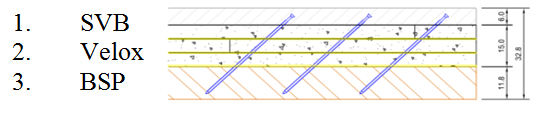
\includegraphics[scale =0.9]{sandwich.png}
\caption{Sandwichaufbau}
\label{sandwichaufbau}
\end{center}
\end{figure}



\section{Verwendete Bauteilkomponenten}
\subsection{Selbstverdichtender Beton, SCC}

Die Verwendung des SCC ist auf seine Vorteile zurückzuführen. Es ist ein besonders fließfähiger Beton, der sich selbst entlüftet und eine ebene Oberfläche bildet. Durch die Fließfähigkeit ist ein besonders guter Verbund mit dem porösem Werstoff,Holzbeton (Velox) gewährleistet. Die Betonschicht wurde auf eine minimale Dicke von 6cm reduziert. Das Limit ergibt sich aus der Verankerungslänge der Schrauben (4 $cm$)und der zuzüglich  Betondeckung von 2 $ cm $. Die Betonrezeptur hat Herr Dipl.Ing. Kirchmayer in den Versuchen ausgearbeitet und wurde von uns übernommen.


\begin{figure}[h]
\begin{center}
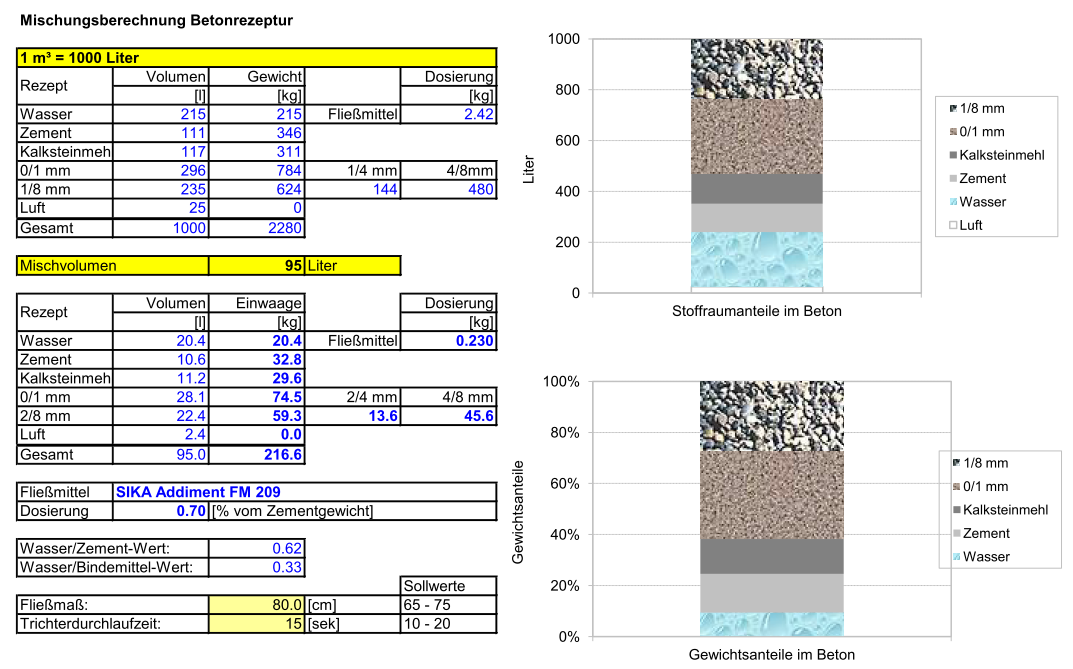
\includegraphics[scale =0.7]{Beton-Mischrezeptur.png}
\caption{Beton-Mischrezeptur [4], mit Okamurarechner}
\label{Beton-Mischrezeptur}
\end{center}
\end{figure}


\subsection{Holzspanbeton}

Holzspanbeton besteht aus den Komponenten Zement, Sägespänen, Wasser, und Additiven und eventuellen Zuschlagstoffen. Die Auswahl des Materials geht auf die Vorversuche von Herrn Kirchmayer bzw. Herrn Schernberger zurück. Die Verwendung der Veloxplatten stellte sich bei der Verarbeitung als sehr gut heraus. Jedoch muss erwähnt werden, dass bei den Versuchen zumeist das Velox versagt hat, und somit auch zusätzliche Verbindungsmittel angewendet werden müssen.
Die Abmessungen der Holzbetonschicht und der Holzplatte ergaben sich aus einem Vielfachen der Dicke der Velox-Platten (50 $mm$) und aus Vorberechnungen mit den FEM-Programm "Sofistik". Die Veloxplatte ist ein Industrieprodukt das ausführlich in der Ausarbeitung von Kirchmayer beschrieben wird.


\begin{figure}[h]
\begin{center}
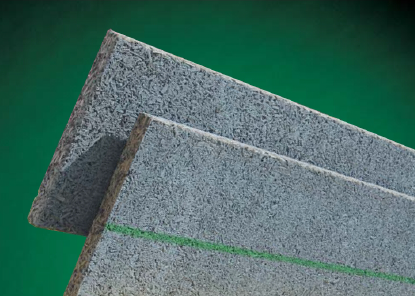
\includegraphics[scale =0.7]{velox.png}
\caption{Holzspanplatte WS 50 der Firma Velox}
\label{velox}
\end{center}
\end{figure}

\subsection{Kreuzlagenholz, CLT}

Die CLt-Platte ist ein flächiges Holzprodukt aus mindestens drei rechtwinkelig zueinander verleimten Schichten. CLT-Produkte zählen zu den Holzmassivbauweisen und können mit großen Abmessungen hergestellt werden. Aufgrund der Vorgabe die Spannweite 7,20m zu Überspannen wurde dieses Produkt gewählt. Es wurde auch schon in den Vorversuchen von Herrn Kirchmayer angewendet und gute Erfahrungen damit gemacht. Die Vorteile hat ebenfalls Herr Kirchmayer in seiner Arbeit schon ausgeabeitet.

Es wurde für alle Großbauteilversuche das Produkt BSP 118 3s DL ind. von der Mayr Mehlfhof  verwendet. In der Abbildung \ref{clt} ist ein Beispielbild einer 5 schichitgen CLT-Platte dargestellt.

\begin{figure}[h]
\begin{center}
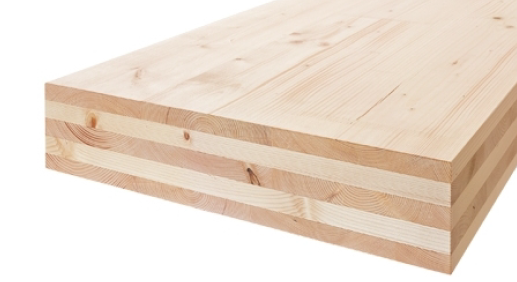
\includegraphics[scale =0.7]{clt.png}
\caption{5 - schichtige Brettsperrholzplatte (CLT)}
\label{clt}
\end{center}
\end{figure}

\subsection{Verbindunsmittel}

Um den Verbund der einzelnen Bauelemente herstellen zu können, kamen verschiedene Verbindungsmittel zur Anwendung. Aus den Vorversuchen von Kirchmayer ist hervorgegangen, dass die besten Verbundergebnisse durch Schrauben und Kleber  erzielt worden sind. Die Verbindungsmittel wurden von uns auch weiter verwendet.




\begin{itemize}
\item Schrauben
\newline
Die verwendeten Schrauben sind durch die Versuche ( siehe Kapitel 2.1) ausgewählt worden.
\newline
\begin{itemize}
\item SFS Intec WR-T-9x400
\end{itemize}

\item Kleber

Die angeführten Kleber im Kaptitel 2.2 Vorversuche beschrieben.
\newline

\begin{itemize}
\item Sikadur-31 AUT Normal Komp. B
\item ElastoCem-109 
\item Sikatop 107 
\end{itemize}

\end{itemize}

\section{Herstellung des Sandwichaufbaus}


\begin{figure}[h!]
	\begin{minipage}[h]{7cm}	
	 Die Herstellung der Versuchskörper war bei allen Proben ident. Wie schon angesprochen 	waren die Verbindungsmittel unterschiedlich angeordnet oder ausgeführt.
	Zu Beginn der Arbeiten haben wir alle Bauteilkomponenten bereitgelegt. Der 					zweikomponenten Kleber wurde mit dem Mischverhältnis, das vom Hersteller angegeben 			wird, abgemischt. Die erste Kleberschicht wurde auf die CLT-Platte aufgetragen. Der 		Auftrag erfolgte mit einer  8 $mm$ Zahnspachtel. Für die Verarbeitungszeit des Klebers 		war laut Datenblatt 45 min Topfzeit vorgegeben. Auf die Kleberschicht wurden die 			Veloxplatten aufgelegt. Dieser Vorgang wiederholte sich zwei mal, um auf die 				vorgegebene Schichtdicke zu kommen
	\end{minipage}
		\hfill
	\begin{minipage}[h]{7cm}
		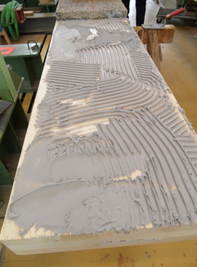
\includegraphics[width=7cm]{kleberauftrag.png}
			\caption{Kleberauftrag auf die CLT-Platte}
			\label{kleberauftrag}
	\end{minipage}
\end{figure}



\begin{figure}[h!]
\begin{minipage}[h]{7cm}
	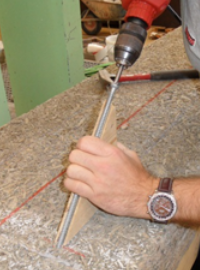
\includegraphics[width=7cm]{einschrauben.png}
	\caption{Einschrauben der Schrauben}
	\label{einschrauben}
\end{minipage}
\hfill
\begin{minipage}[h]{7cm}
Im nächsten Schritt wurde anhand des zuvor angefertigte Bohrmusters auf die obere Veloxschicht gekennzeichnet. Die Schrauben wurden mit einem Hilfswinkel und einem Hammer angesetzt um die geforderten 45 einzuhalten. Die Schrauben wurden anschließend ohne Vorbohren mit einer Bohrmaschine in den Bauteil eingebohrt. Um den Verbund mit dem Beton zu erhalten, stehen die  Schrauben 4 aus dem der oberen Veloxschicht heraus. Dieser Schritt wurde bei dem Bauteil ohne Schrauben nicht gemacht
	
\end{minipage}
\end{figure}

\begin{figure}[h!]
\begin{minipage}[h]{7cm}	
	Der letzte Schritt vor dem betonieren war, dass anbringen der Schalung. Es wurden Schalungsbretter auf eine Höhe von 20 $cm$ zugeschnitten. Die Schalung wurde mit einem Überstand von 6 $cm$ über der letzten Veloxschicht angebracht. Damit man den Überstand allseite gleich erhält, haben wir uns zwei Holzstücke mit den geforderten 6 $cm$ gefertigt. Somit hatte sich das Einrichten der Bretter, einfach gestaltet.  Die Bretter wurden mit Schrauben, die in die Veloxschicht eingeschraubt worden sind, befestigt. Durch die Befestigungsart der Schalung, war das Ausschalen des Trägers mit geringer Arbeit verbunden.

\end{minipage}
\hfill
\begin{minipage}[h]{7cm}
	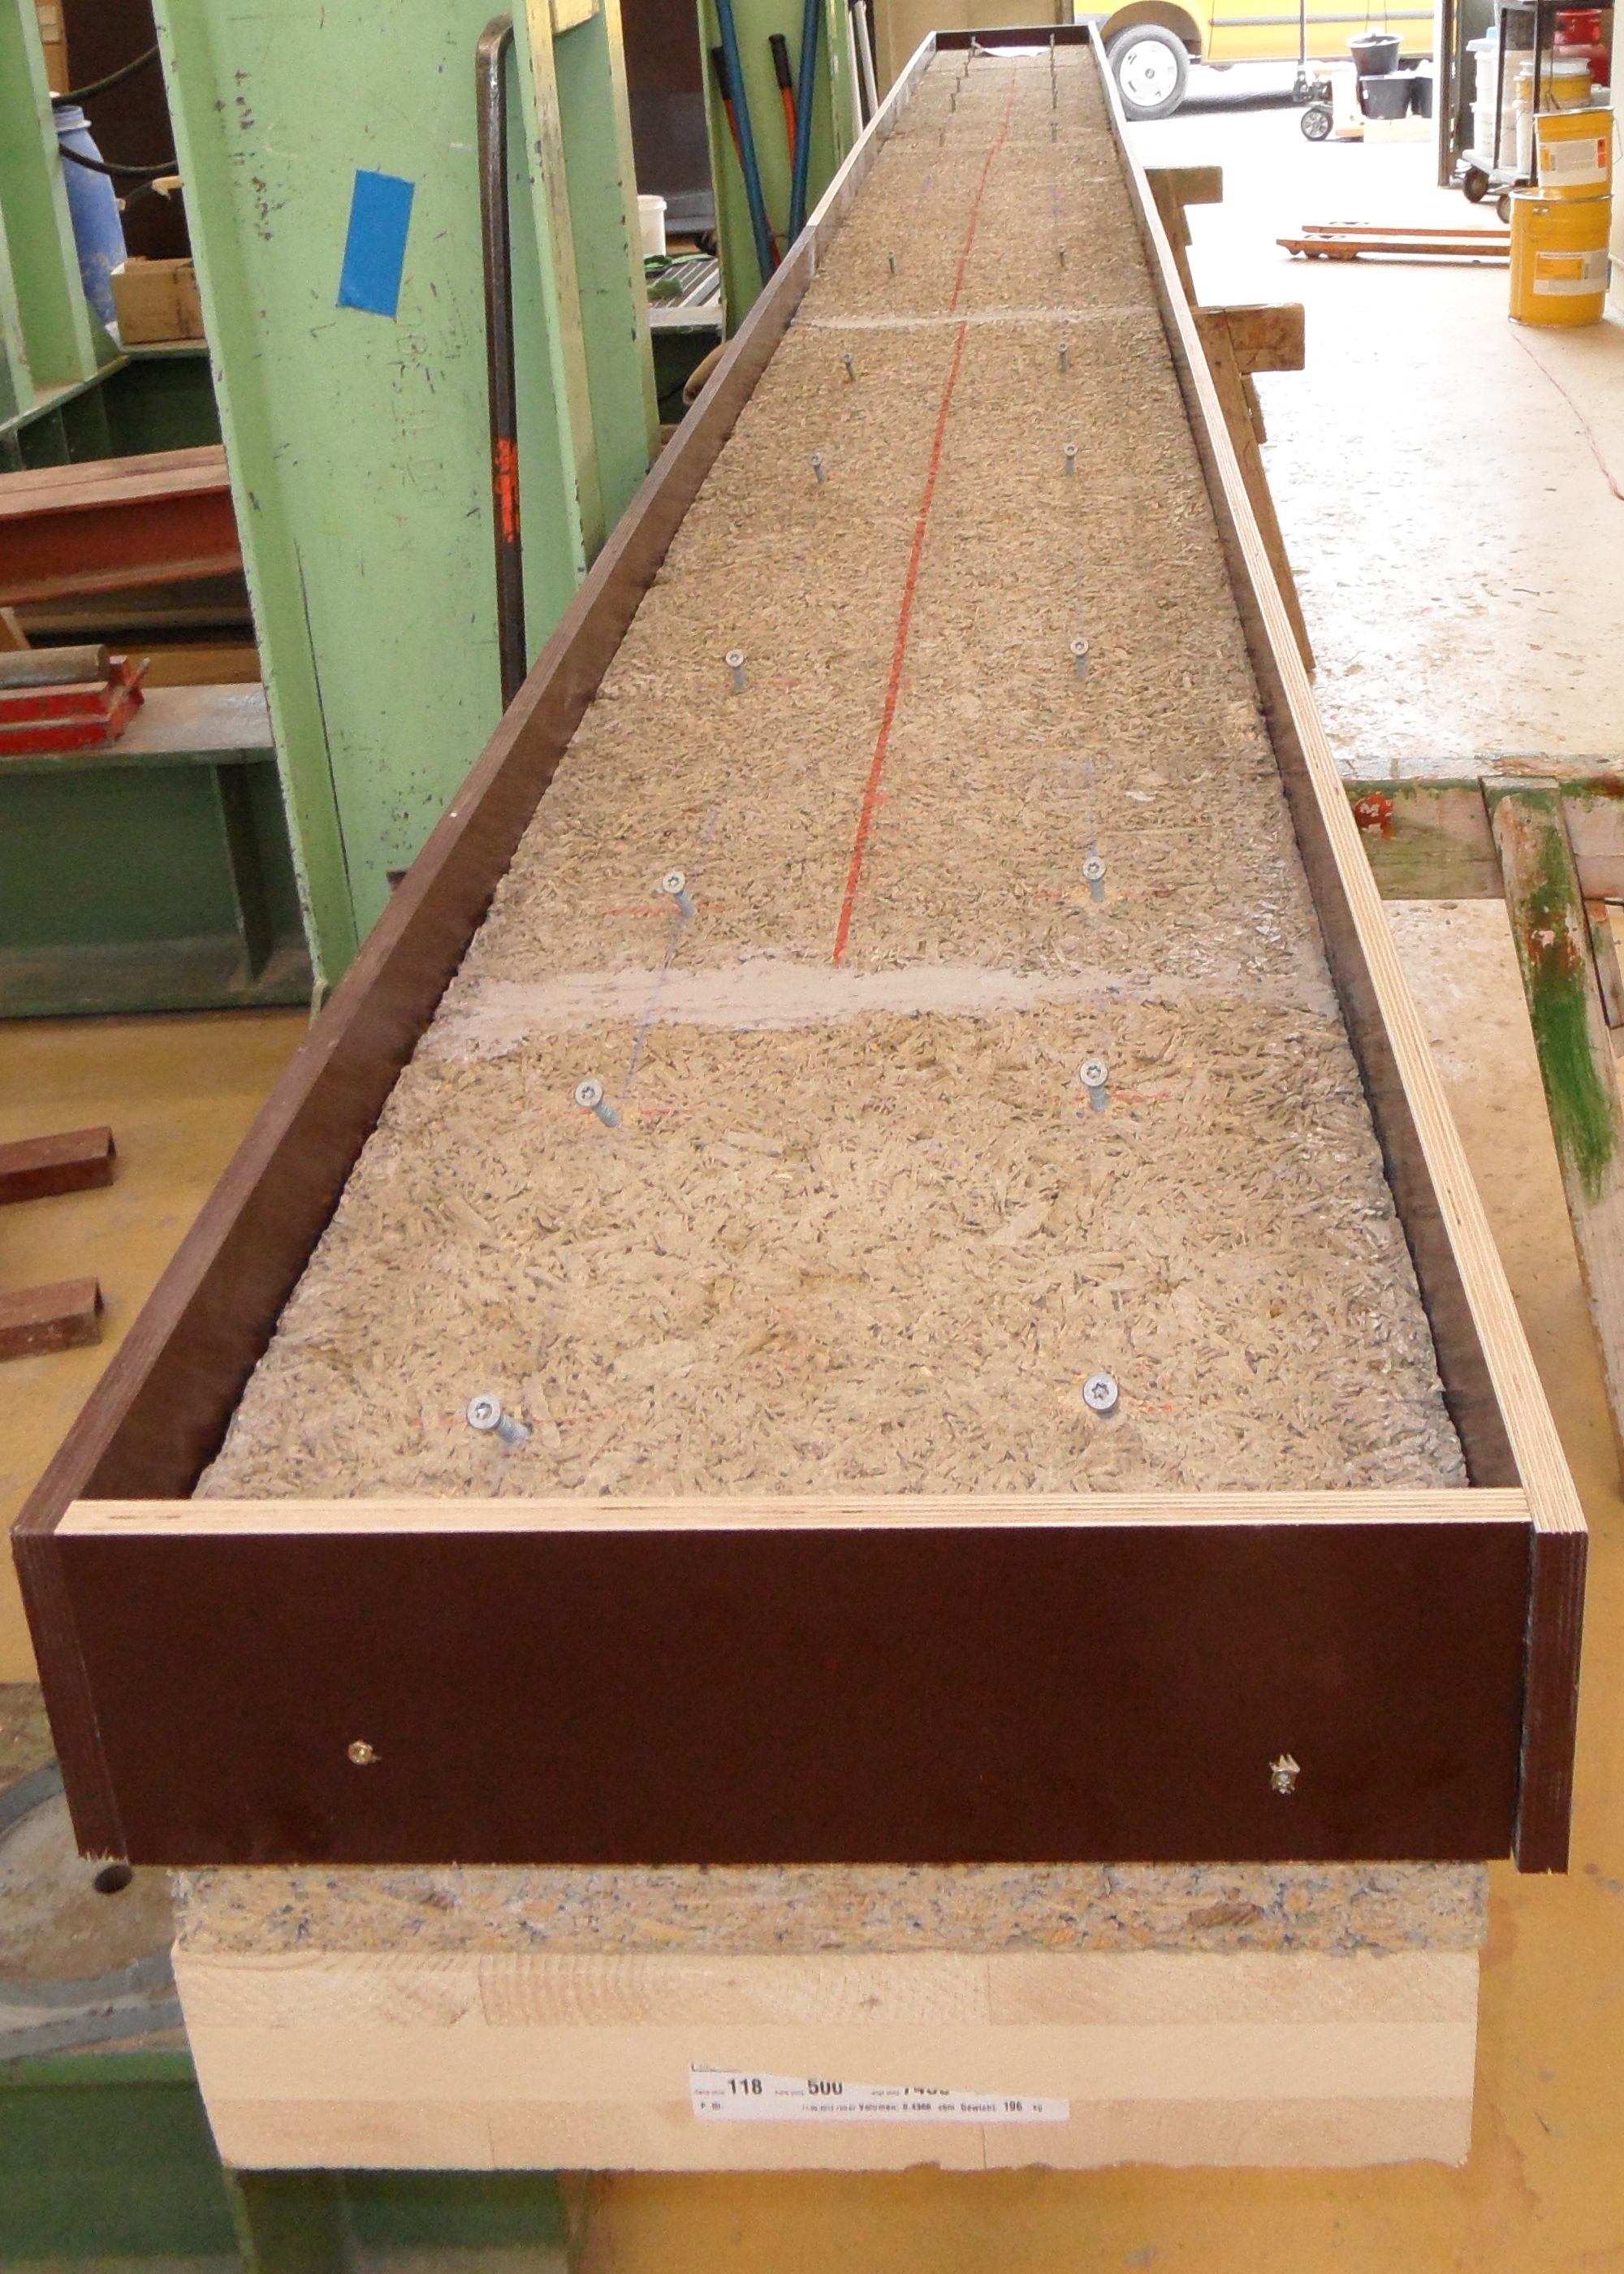
\includegraphics[width=7cm]{einschalen.png}
	\caption{Befestigung der Schalung}
	\label{einschalen}
\end{minipage}
\end{figure}


\begin{figure}[h!]
\begin{minipage}[h]{7cm}
	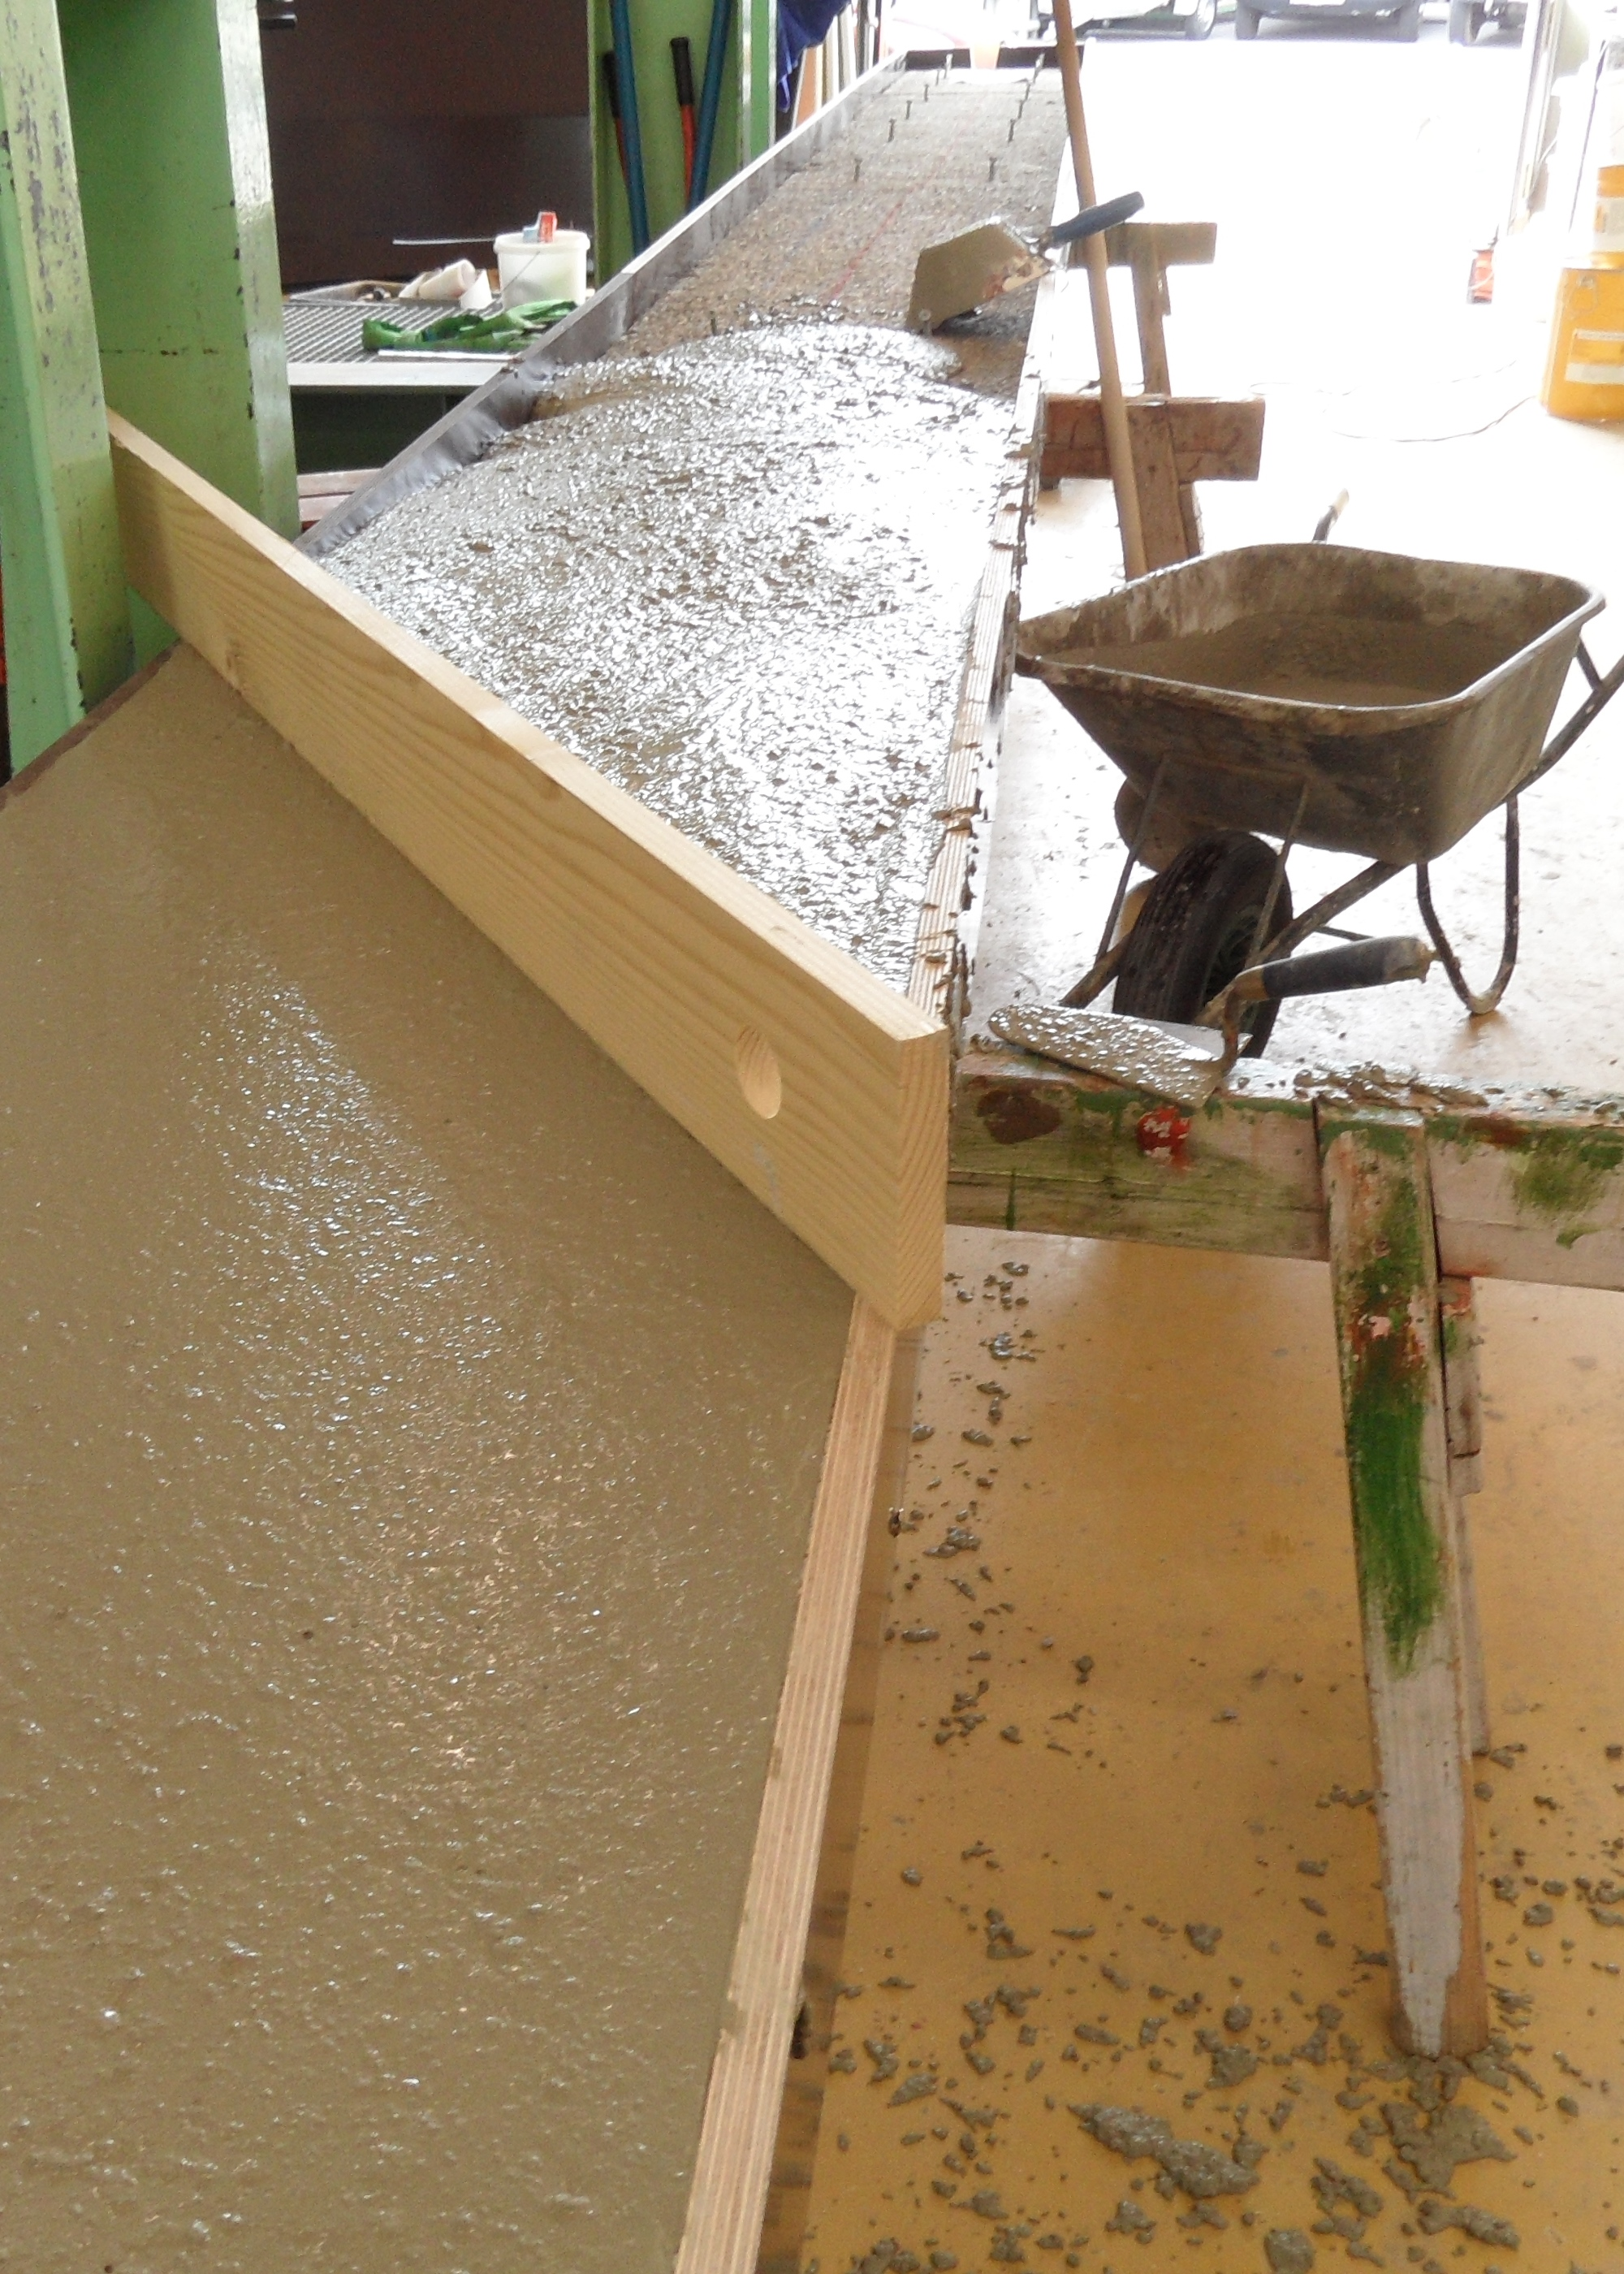
\includegraphics[width=7cm]{betonieren.png}
	\caption{Aufbrinden des SCC}
	\label{betonieren}
\end{minipage}
\hfill
\begin{minipage}[h]{7cm}
Abschließend wurde der Beton hergestellt. Die einzelnen Bestandteile wurden nach der Betonrezeptur [Abbildung: \ref{Beton-Mischrezeptur}] exakte eingewogen und danach mit einem Zwangsmischer vermischt. Der Beton wurde von Hand aufgebracht. Zum Schluss wurde der Beton mit einer Latte abgezogen und mit einem Schwert geglättet.
Für die Lagerung wurden 2 Böcke verwendet, die in den $1/4$ Punkten des Trägers angeordnet worden sind.

	
\end{minipage}
\end{figure}


\chapter{Versuchsaufbau und Durchführung}
Der Versuchsaufbau und die Abmessungen waren bei allen Versuchen wie in der Abbildung \ref{versuchsaufbau} dargestellt.Es handelt sich um einen 4-Punkt-Biegeversuch.   
Beim 4-Punkt-Biegeversuch wird die Prüfprobe auf 2 Auflagen (rote Dreiecke) positioniert und in den $1/4$  Punkten mit der Kraft (F) belastet. Der Vorteil besteht darin, dass zwischen den beiden Krafteinleitungspunkten ein konstantes Biegemoment herrscht. Der Versuchsaufbau ist einfach und er bildet die reale Belastung (Flächenlast) am besten ab. 

\begin{figure}[h]
\begin{center}
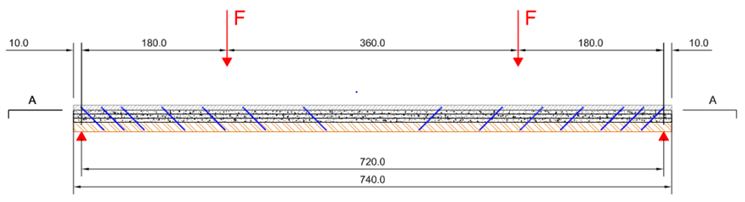
\includegraphics[scale =0.8]{versuchsaufbau.png}
\caption{Versuchsaufbau mit Lagerung und Lasteinleitung}
\label{versuchsaufbau}
\end{center}
\end{figure}

\section{Verwendete Messmittel und deren Anordnung}

Bei dem ersten und zweiten Großbauteilversuch wurde die Verschiebung noch manuell von den Messuhren abgelesen. Bei den Versuchen 3 und 4 wurde Messaufnehmer verwendet, die anschließend beschrieben werden. Die Aufnahme der Verschiebung erfolgte bei allen Versuchen an der gleichen Stelle. Die Messaufnehmer für die Trägerdurchbiegung,wurden in der Trägermitte und unter der Lasteinleitung angeordnet. Weiters wurde auf beiden Trägerenden Messaufnehmer angebracht, um die Verschiebung zwischen Betonschicht und der CLT-Schicht zu messen.

\begin{figure}[h]
\begin{center}
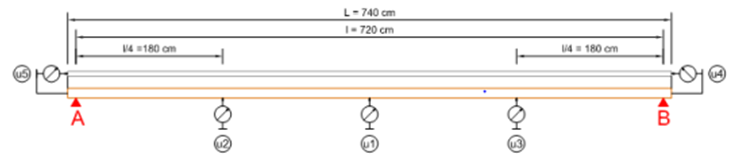
\includegraphics[scale =0.8]{messanordnung.png}
\caption{Anordnung der Messpunkte}
\label{versuchsaufbau}
\end{center}
\end{figure}

In der Abbildung \ref{versuchsaufbau} sind die Messpunkte skizziert und beschriftet.

\begin{figure}[h]
\begin{minipage}[hbt]{8cm}
	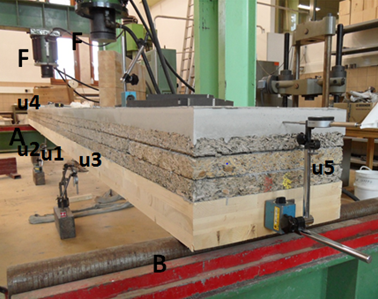
\includegraphics[width=8cm]{messpunkte.png}
	\caption{Mess- und Auflagerpunkte}
	\label{messpunkte}
\end{minipage}
\hfill
\begin{minipage}[hbt]{7cm}
	\begin{itemize}
	\item u1.1/ u1.2: Durchbiegung in Feldmitte 	auf beiden Seiten des Trägers
	\item u2/u3: Durchbiegung bei l/4
	\item u4/u5: Verschiebung der Betonschicht 	gegenüber der Holzschicht an beiden 	Enden des Trägers
	\item u4/u5: Krafteinleitung F ist im l/4 Punkt
	\item A/B Stellen bezeichnend die 	Auflagerpunkte 
	\end{itemize}

	
\end{minipage}
\end{figure}

\section{Wegaufnehmer}	

In diesem Abschnitt werden die die verschiedenen Wegaufnehmer beschrieben.

\subsection{Analoge Wegaufnehmer}

Es wurden analoge Messuhren von der Fa. Käfer verwendet. Die Messuhren besaßen einen Messweg von 7 $cm$ und haben eine Messgenauigkeit von $1/100  mm$. Die Vorrichtung für die vertikale Verschiebung, wurde mit einem Standfuss ausgeführt. Auf den Standfuss wurden die magnetischen Halteeinrichtungen angebracht, welche die Messuhren in der vorgesehenen Position hielten. Der gesamte Aufbau ist in dder Abbildung \ref{messuhr_unten} dargestellt.

Die Befestigung für die horizontale Verschiebung, wurde ebenfalls mit der magnetischen Halteeinrichtung bewerkstelligt. Zuvor musste noch eine Stahlplatte an der CLT-Platte angeschraubt werden, damit die Halteeinrichtung angebracht werden konnte. Der gesamte Aufbau kann der Abbildung \ref{messuhr_seitlich} entnommen werden.

\begin{figure}
\begin{minipage}[h]{6cm}
	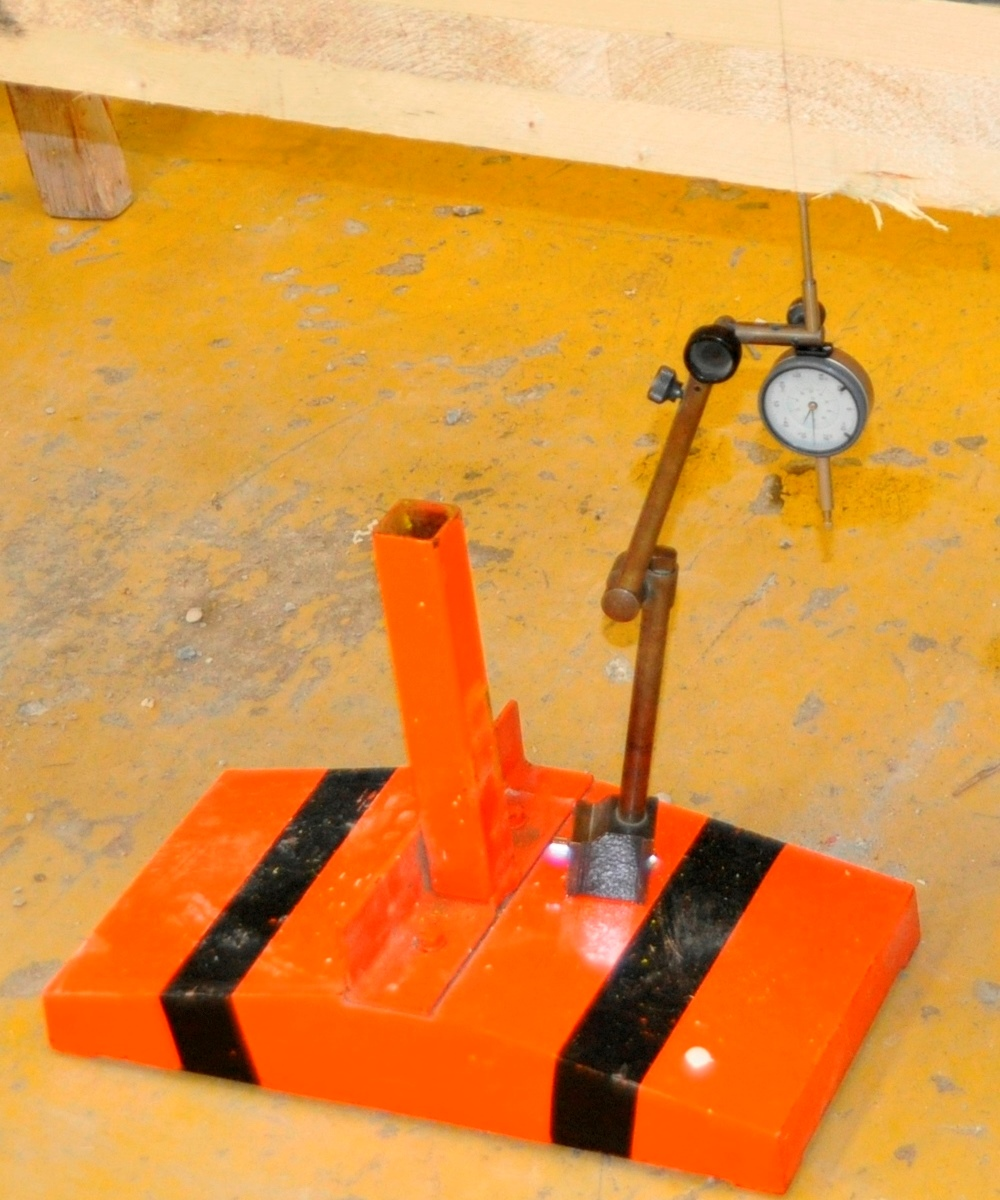
\includegraphics[width=6cm]{messuhr_unten.jpg}
	\caption{Messuhr für vertikale Verschiebung}
	\label{messuhr_unten}
\end{minipage}
\hfill
\begin{minipage}[h]{7cm}
	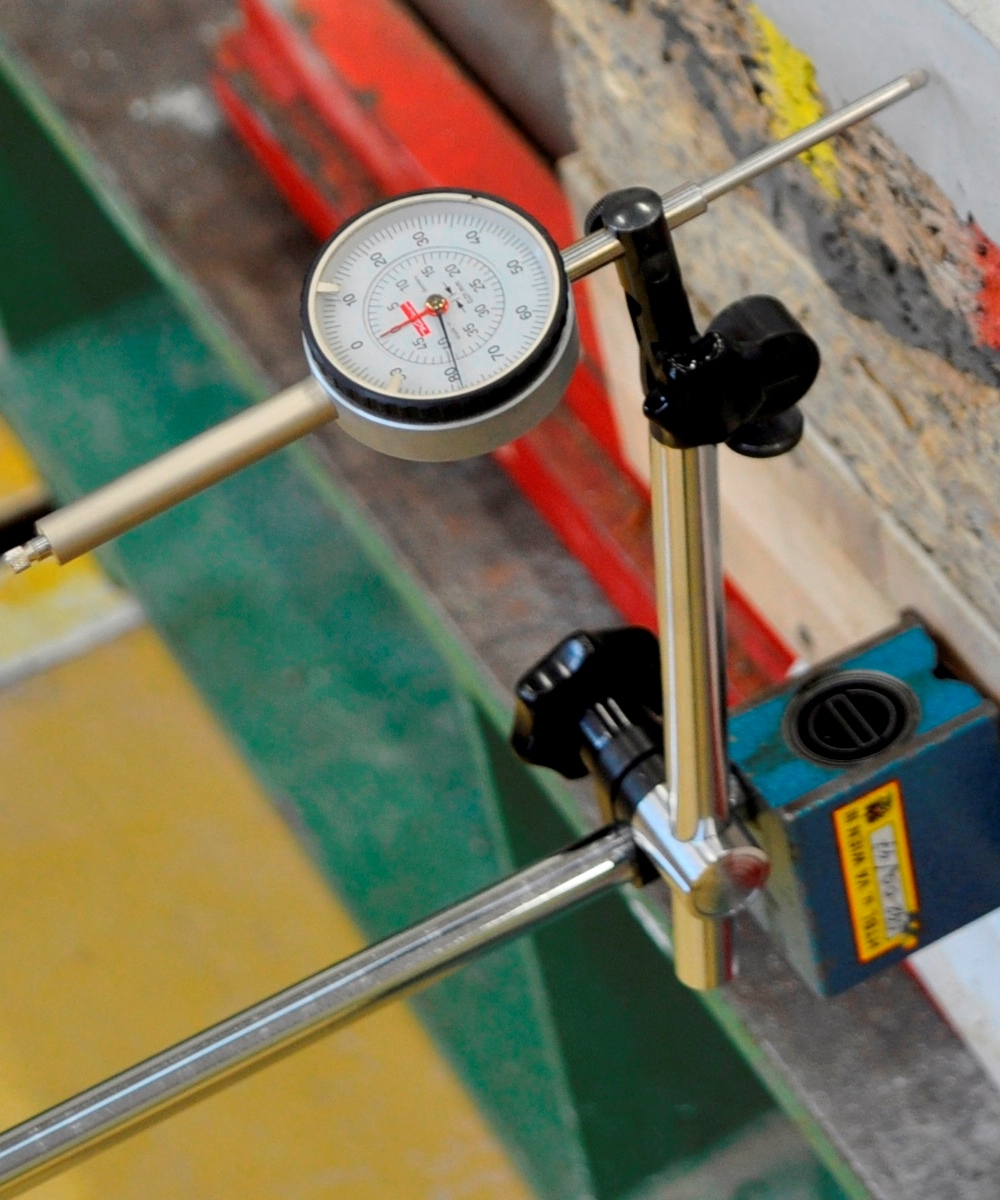
\includegraphics[width=7cm]{messuhr_seitlich.jpg}
	\caption{Messuhr für horizontale Verschiebung}
	\label{messuhr_seitlich}
\end{minipage}
\end{figure}


\subsection{Digitale Wegaufnehmer}

Es wurden digitale Seilzug Wegsensor von der Fa. MICRO-EPSILON verwendet[Serie WDS, Baureihe P60, 1000mm]. Die Messuhren besaßen einen maximalen Messweg von 100 $cm$ und haben eine Messgenauigkeit von $0,024  mm$. Die Vorrichtung für die vertikale Verschiebung, wurde ebenfalls mit dem Standfuss ausgeführt.In den Standfuss wurde die dazugehörige Metallstange eingeführt und mit kleinen Holzkeilen fixiert. Der  Wegsonsor wurde mit M4 Schrauben, Flügelmuttern und einer Holzplatte an der Metallstange montiert. Um das Seil auf der Messposition zu halten wurde eine Schraube in die CLT-Platte eingeschraubt. Der gesamte Aufbau ist in der Abbildung \ref{d_aufnehmer_unten} dargestellt.

Für die Messung der horizontalen Verschiebung, wurde eine Vorrichtung zusammengeschweißt. Die Vorrichung musste nur noch mit Schrauben auf der CLT-Platte angeschraubt werden. Der Wegsensor wurde ebenfalls mit M4 Schrauben, Flügelmuttern und einer Holzplatte, an der Vorrichung befestigt. Der gesamte Aufbau kann aus der Abbildung \ref{messuhr_seitlich} entnommen werden.



\begin{figure}[h!]
\begin{minipage}[h!]{5cm}
	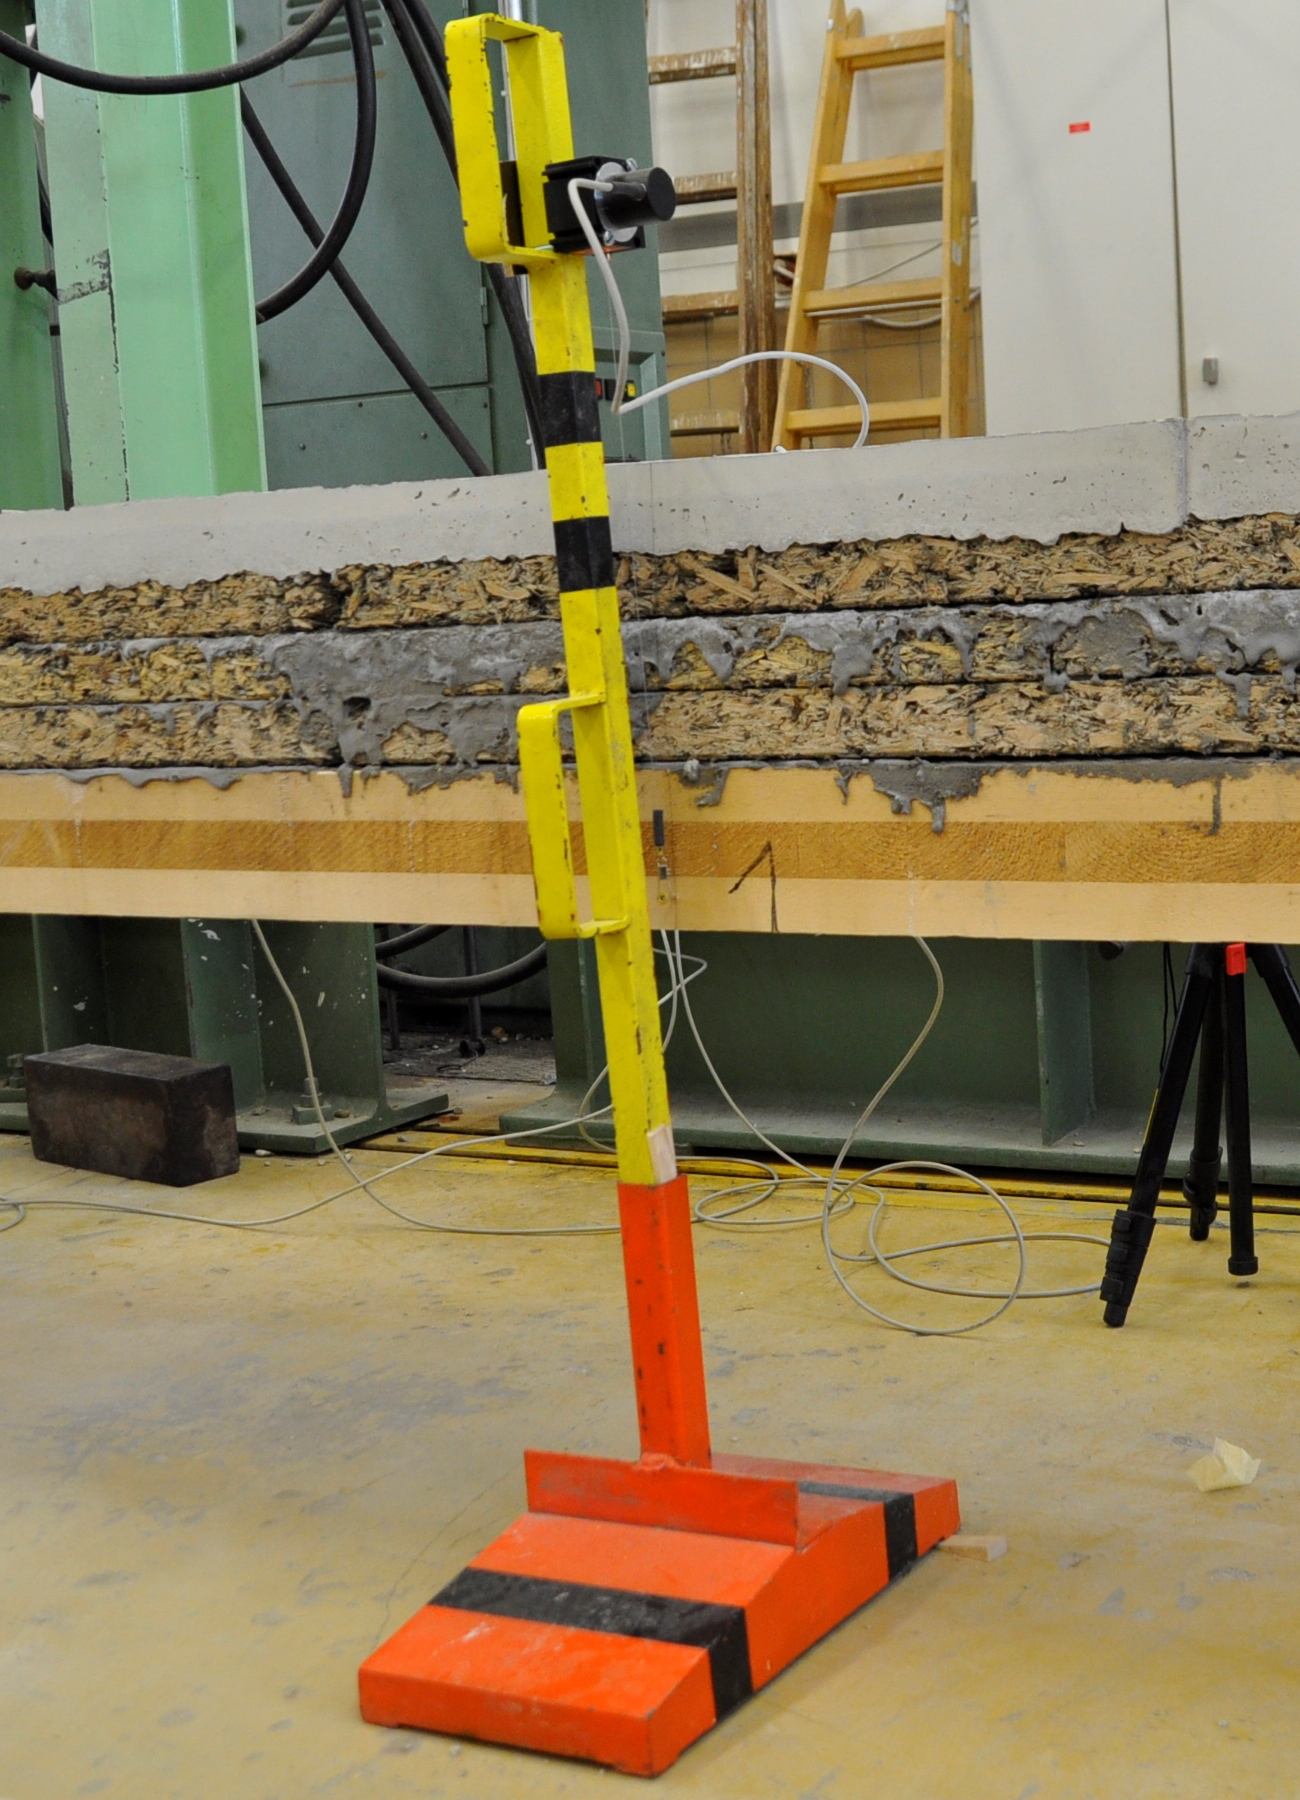
\includegraphics[width=5cm]{d_aufnehmer_unten.jpg}
	\caption{Messaufnehmer für vertikale Verschiebung}
	\label{d_aufnehmer_unten}
\end{minipage}
\hfill
\begin{minipage}[h!]{5cm}
	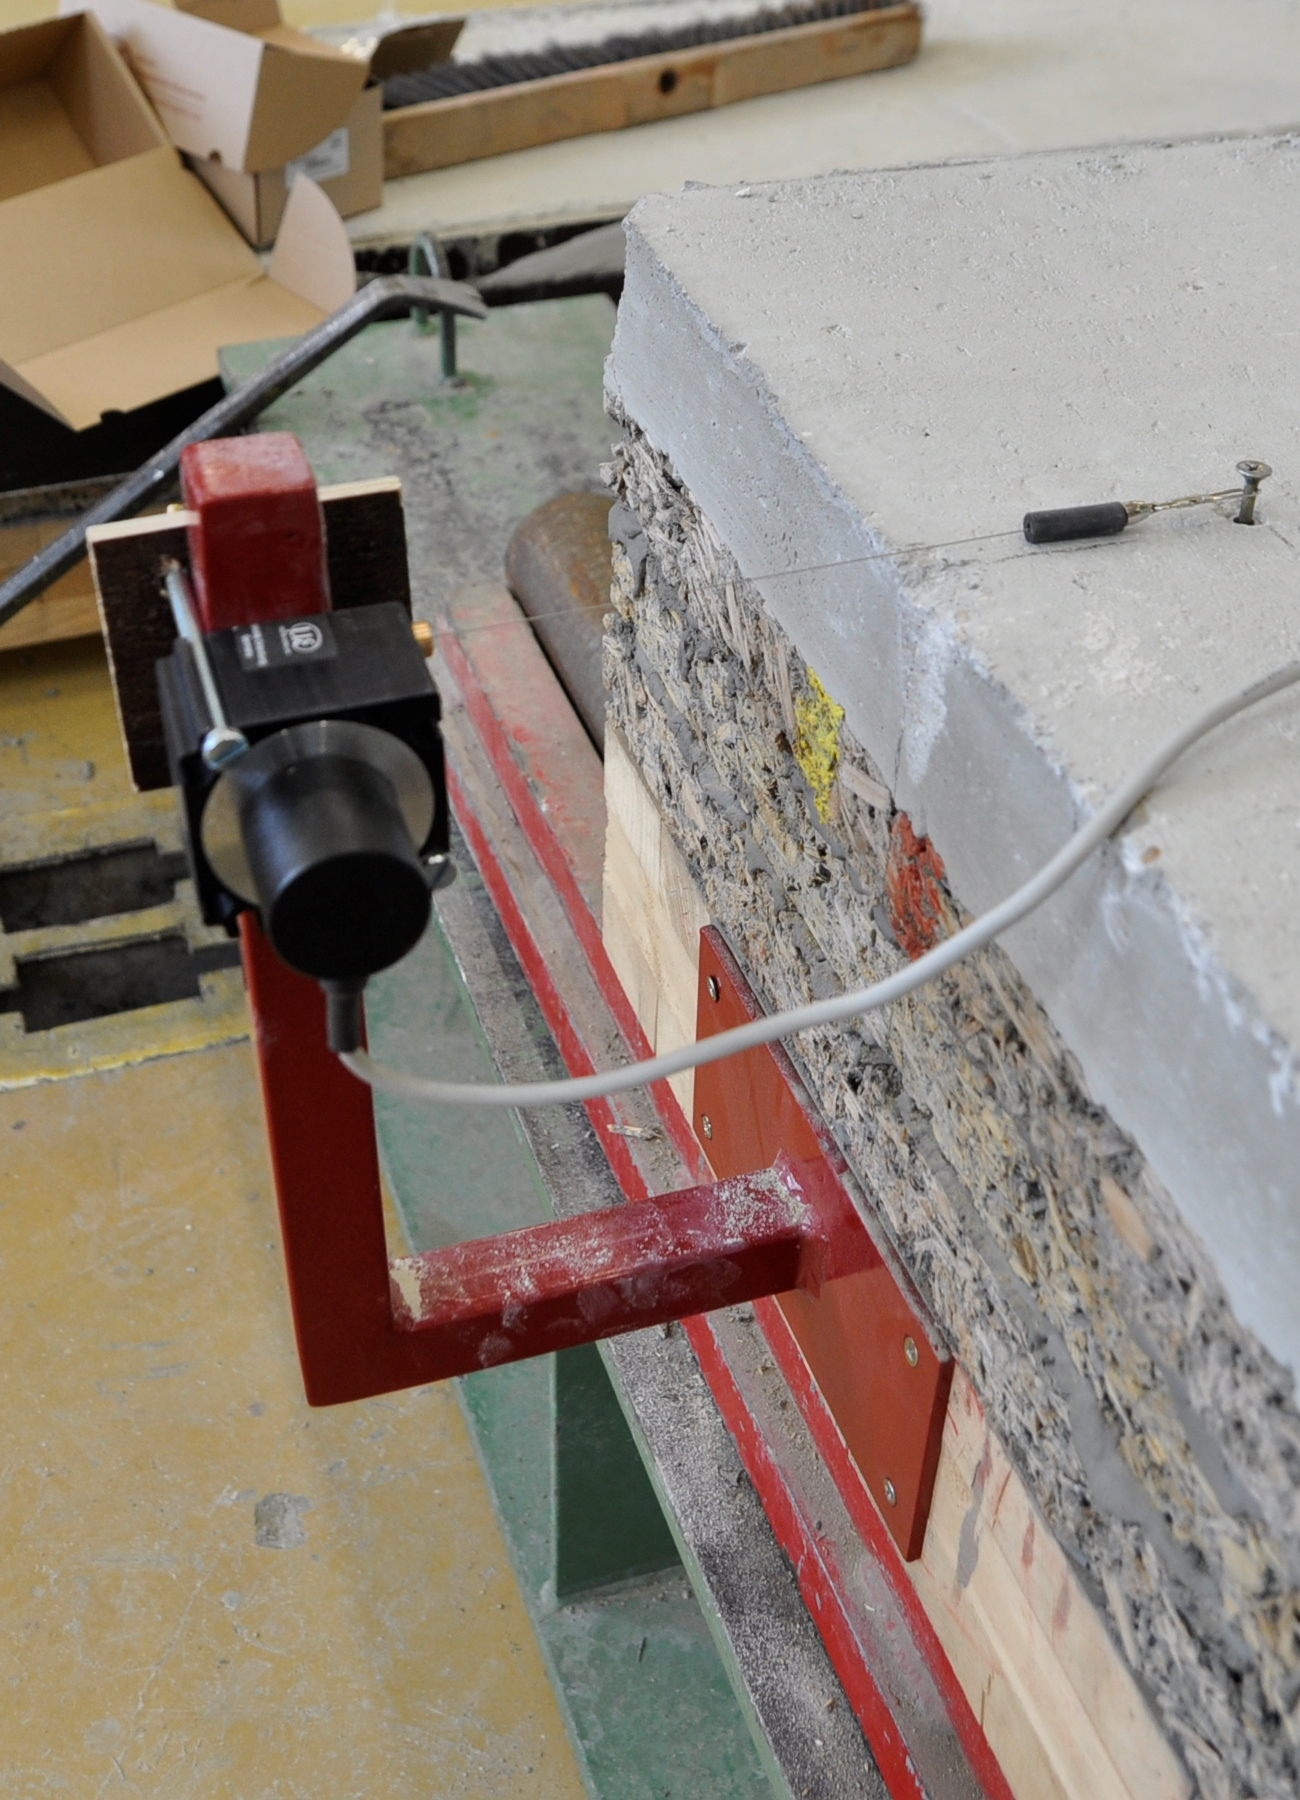
\includegraphics[width=5cm]{d_aufnehmer_seitlich.jpg}
	\caption{Messaufnehmer für horizontale Verschiebung}
	\label{d_aufnehmer_seitlich}
\end{minipage}
\end{figure}










	
\section{Durchführung des Versuchs}
Es wurde ein Versuch an einem Einfeldträger mit 4 Punkt Biegeverfahren durchgeführt. Die Lasteinleitung befand sich im viertel Punkt des Trägers, in der Mitte der Trägerbreite. Der Aufbau des Versuchs bzw. die Abmessungen des Bauteils ist in der Abbildung \ref{versuchsaufbau} zu entnehmen. Die Belastungsgeschwindigkeit für die Bauteilversuche 1 und 2 wurde mit 4 $kN/min$ gewählt.Das Ablesen erfolgte in Schritten von 2$kN$. Bei den Bauteilversuchen 3 und 4 wurde eine vorgegebene Belastungskurve gewählt. Die Kurve wurde der Norm ÖN EN 380 entnommen. Das Grundverfahren der Belastung besteht aus den 7 Verfahrensstufen. 

\paragraph{Belastungserklärung}
\begin{itemize}
\item $G_{2}$\ldots ist der zusätzlich erforderliche Aufbau (Dämmung, Estrich, Bodenbelag
\item $Q$ \ldots ist die veränderliche Last lt. EC1 für Wohnräume
\item Belastungsgeschwindigkeit: 1,5 $kN/min$
\item Die Lastangaben beziehen sich auf die Kraft pro Zylinder.
\end{itemize}
	

\begin{figure}
\begin{center}

	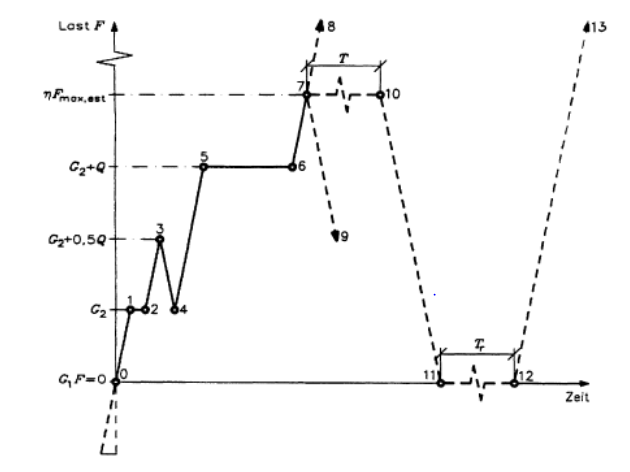
\includegraphics[width=12cm]{belastungskurve.png}
	\caption{Schematische Belasungskurve}
	\label{belastungskurve}

\end{center}	
\end{figure}	

\begin{table}
\caption{Grundlagen der Belastung}
\begin{center}
\begin{tabular}{|c|c|c|c|}
\hline 
Verfahrensstufe & Belastungsverfahren & Zeit in [s] & F [kN] \\ 
\hline \hline
0 & Es wirkt nur G;F=0 &  &  \\ 
\hline 
0-1 & F=G aufbringen &  & 2,70 \\ 
\hline 
1-2 & F=G konstant halten & 120 & 2,70 \\ 
\hline 
2-3 & F=G+0,5*Q aufbringen & 120 & 5,40 \\ 
\hline 
3-4 & 0,5 Q entlasten & 120 & 2,70 \\ 
\hline 
4-5 & F=G+Q aufbringen & 240 & 8,10 \\ 
\hline 
5-6 & F=G+Q konstant halten & 600 & 8,10 \\ 
\hline 
6-8 & F= steigern bis Bruch &  &  \\ 
\hline \hline
\multicolumn{4}{|c|}{ max. Belastungsgeschwindigkeit 0,25Q je 60 sec} \\ 
\hline 
\end{tabular} 
\label{tab:belastung}
\end{center}
\end{table}

















	
	
	




\end{document}



